\documentclass[]{article}
\usepackage{lmodern}
\usepackage{amssymb,amsmath}
\usepackage{ifxetex,ifluatex}
\usepackage{fixltx2e} % provides \textsubscript
\ifnum 0\ifxetex 1\fi\ifluatex 1\fi=0 % if pdftex
  \usepackage[T1]{fontenc}
  \usepackage[utf8]{inputenc}
\else % if luatex or xelatex
  \ifxetex
    \usepackage{mathspec}
  \else
    \usepackage{fontspec}
  \fi
  \defaultfontfeatures{Ligatures=TeX,Scale=MatchLowercase}
\fi
% use upquote if available, for straight quotes in verbatim environments
\IfFileExists{upquote.sty}{\usepackage{upquote}}{}
% use microtype if available
\IfFileExists{microtype.sty}{%
\usepackage[]{microtype}
\UseMicrotypeSet[protrusion]{basicmath} % disable protrusion for tt fonts
}{}
\PassOptionsToPackage{hyphens}{url} % url is loaded by hyperref
\usepackage[unicode=true]{hyperref}
\hypersetup{
            pdftitle={Chemical patterns of colony membership and mother-offspring similarity in Antarctic fur seals are reproducible - R Code},
            pdfauthor={Jonas Tebbe, Emily Humble, Martin A. Stoffel, Lisa Johanna Tewes, Caroline Müller, Jaume Forcada, Barbara Caspers \& Joseph Ivan Hoffman},
            pdfborder={0 0 0},
            breaklinks=true}
\urlstyle{same}  % don't use monospace font for urls
\usepackage[margin=1in]{geometry}
\usepackage{color}
\usepackage{fancyvrb}
\newcommand{\VerbBar}{|}
\newcommand{\VERB}{\Verb[commandchars=\\\{\}]}
\DefineVerbatimEnvironment{Highlighting}{Verbatim}{commandchars=\\\{\}}
% Add ',fontsize=\small' for more characters per line
\usepackage{framed}
\definecolor{shadecolor}{RGB}{248,248,248}
\newenvironment{Shaded}{\begin{snugshade}}{\end{snugshade}}
\newcommand{\KeywordTok}[1]{\textcolor[rgb]{0.13,0.29,0.53}{\textbf{#1}}}
\newcommand{\DataTypeTok}[1]{\textcolor[rgb]{0.13,0.29,0.53}{#1}}
\newcommand{\DecValTok}[1]{\textcolor[rgb]{0.00,0.00,0.81}{#1}}
\newcommand{\BaseNTok}[1]{\textcolor[rgb]{0.00,0.00,0.81}{#1}}
\newcommand{\FloatTok}[1]{\textcolor[rgb]{0.00,0.00,0.81}{#1}}
\newcommand{\ConstantTok}[1]{\textcolor[rgb]{0.00,0.00,0.00}{#1}}
\newcommand{\CharTok}[1]{\textcolor[rgb]{0.31,0.60,0.02}{#1}}
\newcommand{\SpecialCharTok}[1]{\textcolor[rgb]{0.00,0.00,0.00}{#1}}
\newcommand{\StringTok}[1]{\textcolor[rgb]{0.31,0.60,0.02}{#1}}
\newcommand{\VerbatimStringTok}[1]{\textcolor[rgb]{0.31,0.60,0.02}{#1}}
\newcommand{\SpecialStringTok}[1]{\textcolor[rgb]{0.31,0.60,0.02}{#1}}
\newcommand{\ImportTok}[1]{#1}
\newcommand{\CommentTok}[1]{\textcolor[rgb]{0.56,0.35,0.01}{\textit{#1}}}
\newcommand{\DocumentationTok}[1]{\textcolor[rgb]{0.56,0.35,0.01}{\textbf{\textit{#1}}}}
\newcommand{\AnnotationTok}[1]{\textcolor[rgb]{0.56,0.35,0.01}{\textbf{\textit{#1}}}}
\newcommand{\CommentVarTok}[1]{\textcolor[rgb]{0.56,0.35,0.01}{\textbf{\textit{#1}}}}
\newcommand{\OtherTok}[1]{\textcolor[rgb]{0.56,0.35,0.01}{#1}}
\newcommand{\FunctionTok}[1]{\textcolor[rgb]{0.00,0.00,0.00}{#1}}
\newcommand{\VariableTok}[1]{\textcolor[rgb]{0.00,0.00,0.00}{#1}}
\newcommand{\ControlFlowTok}[1]{\textcolor[rgb]{0.13,0.29,0.53}{\textbf{#1}}}
\newcommand{\OperatorTok}[1]{\textcolor[rgb]{0.81,0.36,0.00}{\textbf{#1}}}
\newcommand{\BuiltInTok}[1]{#1}
\newcommand{\ExtensionTok}[1]{#1}
\newcommand{\PreprocessorTok}[1]{\textcolor[rgb]{0.56,0.35,0.01}{\textit{#1}}}
\newcommand{\AttributeTok}[1]{\textcolor[rgb]{0.77,0.63,0.00}{#1}}
\newcommand{\RegionMarkerTok}[1]{#1}
\newcommand{\InformationTok}[1]{\textcolor[rgb]{0.56,0.35,0.01}{\textbf{\textit{#1}}}}
\newcommand{\WarningTok}[1]{\textcolor[rgb]{0.56,0.35,0.01}{\textbf{\textit{#1}}}}
\newcommand{\AlertTok}[1]{\textcolor[rgb]{0.94,0.16,0.16}{#1}}
\newcommand{\ErrorTok}[1]{\textcolor[rgb]{0.64,0.00,0.00}{\textbf{#1}}}
\newcommand{\NormalTok}[1]{#1}
\usepackage{graphicx,grffile}
\makeatletter
\def\maxwidth{\ifdim\Gin@nat@width>\linewidth\linewidth\else\Gin@nat@width\fi}
\def\maxheight{\ifdim\Gin@nat@height>\textheight\textheight\else\Gin@nat@height\fi}
\makeatother
% Scale images if necessary, so that they will not overflow the page
% margins by default, and it is still possible to overwrite the defaults
% using explicit options in \includegraphics[width, height, ...]{}
\setkeys{Gin}{width=\maxwidth,height=\maxheight,keepaspectratio}
\IfFileExists{parskip.sty}{%
\usepackage{parskip}
}{% else
\setlength{\parindent}{0pt}
\setlength{\parskip}{6pt plus 2pt minus 1pt}
}
\setlength{\emergencystretch}{3em}  % prevent overfull lines
\providecommand{\tightlist}{%
  \setlength{\itemsep}{0pt}\setlength{\parskip}{0pt}}
\setcounter{secnumdepth}{0}
% Redefines (sub)paragraphs to behave more like sections
\ifx\paragraph\undefined\else
\let\oldparagraph\paragraph
\renewcommand{\paragraph}[1]{\oldparagraph{#1}\mbox{}}
\fi
\ifx\subparagraph\undefined\else
\let\oldsubparagraph\subparagraph
\renewcommand{\subparagraph}[1]{\oldsubparagraph{#1}\mbox{}}
\fi

% set default figure placement to htbp
\makeatletter
\def\fps@figure{htbp}
\makeatother


\title{Chemical patterns of colony membership and mother-offspring similarity
in Antarctic fur seals are reproducible - R Code}
\author{Jonas Tebbe, Emily Humble, Martin A. Stoffel, Lisa Johanna Tewes,
Caroline Müller, Jaume Forcada, Barbara Caspers \& Joseph Ivan Hoffman}
\date{April 2020}

\begin{document}
\maketitle

\subsection{Used packages}\label{used-packages}

Install with ``install.packages''. After installation, packages can be
called with `library' oder `require'

\begin{Shaded}
\begin{Highlighting}[]
\KeywordTok{library}\NormalTok{(GCalignR)}
\KeywordTok{library}\NormalTok{(vegan)}
\KeywordTok{library}\NormalTok{(readr)}
\KeywordTok{library}\NormalTok{(ggplot2)}
\KeywordTok{library}\NormalTok{(ggbeeswarm)}
\KeywordTok{library}\NormalTok{(tidyverse)}
\KeywordTok{library}\NormalTok{(pairwiseAdonis)}
\end{Highlighting}
\end{Shaded}

\subsection{Alignment procedure}\label{alignment-procedure}

\begin{Shaded}
\begin{Highlighting}[]
\NormalTok{## Alignment protocol to align a data frame with GCMS peaks for mother-pup pairs and pure pup colonies. For comparability, the six colonies only include pure pup data and thus, need a different alignment protocol, as algorithm properties are inherited within the function but not across functions callings. In consequence, alignment is more accurate for a set data subset.}


\KeywordTok{load}\NormalTok{(}\StringTok{"RData/objects/seal_raw_dfs.Rdata"}\NormalTok{)}

\CommentTok{# index correct MP & pup_colony subset}
\NormalTok{index_MP <-}\StringTok{ }\KeywordTok{c}\NormalTok{(}\DecValTok{1}\OperatorTok{:}\DecValTok{61}\NormalTok{,}\DecValTok{72}\OperatorTok{:}\DecValTok{111}\NormalTok{)}
\NormalTok{index_pupcols <-}\StringTok{ }\KeywordTok{c}\NormalTok{(}\DecValTok{51}\OperatorTok{:}\DecValTok{160}\NormalTok{)}

\CommentTok{# Aligning mom-pup colonies}
\NormalTok{mom_pup_aligned <-}\StringTok{ }\KeywordTok{align_chromatograms}\NormalTok{(}\DataTypeTok{data =}\NormalTok{ all_dfs[index_MP], }\CommentTok{# input data}
                                         \DataTypeTok{rt_col_name =} \StringTok{"RT"}\NormalTok{, }\CommentTok{# retention time variable name }
                                         \DataTypeTok{rt_cutoff_low =} \DecValTok{15}\NormalTok{, }\CommentTok{# remove peaks below 15 Minutes}
                                         \DataTypeTok{rt_cutoff_high =} \FloatTok{54.7}\NormalTok{, }\CommentTok{# remove peaks exceeding 54.7 Minutes}
                                         \DataTypeTok{reference =} \StringTok{"P13"}\NormalTok{, }\CommentTok{# sample with highest overall peak number}
                                         \DataTypeTok{max_linear_shift =} \FloatTok{0.05}\NormalTok{, }\CommentTok{# Premise 1: max. shift for linear corrections}
                                         \DataTypeTok{max_diff_peak2mean =} \FloatTok{0.08}\NormalTok{, }\CommentTok{# Premise 2: max. distance of a peak to the mean across samples}
                                         \DataTypeTok{min_diff_peak2peak =} \FloatTok{0.03}\NormalTok{, }\CommentTok{# Premise 3: min. expected distance between peaks }
                                         \DataTypeTok{delete_single_peak =}\NormalTok{ T, }\CommentTok{# delete peaks that are present in just one sample }
                                         \DataTypeTok{write_output =} \OtherTok{NULL}\NormalTok{) }\CommentTok{# add variable names to write aligned data to text files}

\CommentTok{# Aligning six pup colonies}
\NormalTok{pup_colonies_aligned <-}\StringTok{ }\KeywordTok{align_chromatograms}\NormalTok{(}\DataTypeTok{data =}\NormalTok{ all_dfs[index_pupcols], }\CommentTok{# input data}
                                         \DataTypeTok{rt_col_name =} \StringTok{"RT"}\NormalTok{, }\CommentTok{# retention time variable name }
                                         \DataTypeTok{rt_cutoff_low =} \DecValTok{15}\NormalTok{, }\CommentTok{# remove peaks below 15 Minutes}
                                         \DataTypeTok{rt_cutoff_high =} \FloatTok{54.7}\NormalTok{, }\CommentTok{# remove peaks exceeding 54.7 Minutes}
                                         \DataTypeTok{reference =} \StringTok{"P13"}\NormalTok{,}\CommentTok{# sample with highest overall peak number }
                                         \DataTypeTok{max_linear_shift =} \FloatTok{0.05}\NormalTok{, }\CommentTok{# Premise 1: max. shift for linear corrections}
                                         \DataTypeTok{max_diff_peak2mean =} \FloatTok{0.08}\NormalTok{, }\CommentTok{# Premise 2: max. distance of a peak to the mean across samples}
                                         \DataTypeTok{min_diff_peak2peak =} \FloatTok{0.03}\NormalTok{, }\CommentTok{# Premise 3: min. expected distance between peaks}
                                         \DataTypeTok{delete_single_peak =}\NormalTok{ T, }\CommentTok{# delete peaks that are present in just one sample }
                                         \DataTypeTok{write_output =} \OtherTok{NULL}\NormalTok{) }\CommentTok{# add variable names to write aligned data to text files}
\end{Highlighting}
\end{Shaded}

\subsection{Alignment and preliminary data
properties}\label{alignment-and-preliminary-data-properties}

\begin{Shaded}
\begin{Highlighting}[]
\NormalTok{## Load and view GCalignR alignment objects for GCMS scent data }
\NormalTok{## in two and six breeding beaches}
\KeywordTok{load}\NormalTok{(}\StringTok{"RData/objects/mom_pup_alignment_GCalignR.RData"}\NormalTok{)}
\NormalTok{mom_pup_aligned}
\end{Highlighting}
\end{Shaded}

\begin{verbatim}
## Summary of Peak Alignment running align_chromatograms
## Input: all_dfs[index2]
## Start:  2019-05-21 11:41:08  Finished:  2019-05-21 11:44:23 
## 
## Call:
##   GCalignR::align_chromatograms(data=[, data=all_dfs, data=index2, rt_col_name=RT,
##   rt_cutoff_low=15, rt_cutoff_high=54.7, reference=P13, max_linear_shift=0.05,
##   max_diff_peak2mean=0.08, min_diff_peak2peak=0.03, delete_single_peak=T,
##   sep=\t, ...=)
## 
## Summary of scored substances:
##    total singular retained 
##      157       39      118 
## 
## In total 157 substances were identified among all samples. 39 substances were
##   present in just one single sample and were removed. 118 substances are retained
##   after all filtering steps.
## 
## Sample overview:
##   The following 101 samples were aligned to the reference 'P13':
##   M01, M02, M03, M04, M05, M06, M07, M08, M09, M10, M11, M12, M13, M14, M15, M16,
##   M17, M18, M19, M20, M21, M22, M23, M24, M25, M26, M27, M28, M29, M30, M31, M32,
##   M33, M34, M35, M36, M37, M38, M39, M40, M41, M42, M43, M44, M45, M46, M47, M48,
##   M49, M50, P01, P02, P03, P04, P05, P06, P07, P07b, P08, P09, P10, P11, P12, P13,
##   P14, P15, P16, P17, P18, P19, P20, P21, P22, P23, P24, P25, P26, P27, P28, P29,
##   P30, P31, P32, P33, P34, P35, P36, P37, P38, P39, P40, P41, P42, P43, P44, P45,
##   P46, P47, P48, P49, P50
## 
## For further details type:
##   'gc_heatmap(x)' to retrieve heatmaps
##   'plot(x)' to retrieve further diagnostic plots
\end{verbatim}

\begin{Shaded}
\begin{Highlighting}[]
\KeywordTok{load}\NormalTok{(}\StringTok{"RData/objects/pup_colonies_alignment_GCalignR.RData"}\NormalTok{)}
\NormalTok{pup_colonies_aligned}
\end{Highlighting}
\end{Shaded}

\begin{verbatim}
## Summary of Peak Alignment running align_chromatograms
## Input: all_dfs[index4]
## Start:  2019-05-23 11:36:39  Finished:  2019-05-23 11:40:15 
## 
## Call:
##   GCalignR::align_chromatograms(data=[, data=all_dfs, data=index4, rt_col_name=RT,
##   rt_cutoff_low=15, rt_cutoff_high=54.7, reference=P13, max_linear_shift=0.05,
##   max_diff_peak2mean=0.08, min_diff_peak2peak=0.03, delete_single_peak=T,
##   sep=\t, ...=)
## 
## Summary of scored substances:
##    total singular retained 
##      143       28      115 
## 
## In total 143 substances were identified among all samples. 28 substances were
##   present in just one single sample and were removed. 115 substances are retained
##   after all filtering steps.
## 
## Sample overview:
##   The following 110 samples were aligned to the reference 'P13':
##   P01, P02, P03, P04, P05, P06, P07, P07b, P08, P09, P10, P100, P101, P102, P103,
##   P104, P105, P106, P107, P108, P109, P11, P12, P13, P14, P15, P16, P17, P18, P19,
##   P20, P21, P22, P23, P24, P25, P26, P27, P28, P29, P30, P31, P32, P33, P34, P35,
##   P36, P37, P38, P39, P40, P41, P42, P43, P44, P45, P46, P47, P48, P49, P50, P51,
##   P52, P53, P54, P55, P56, P57, P58, P59, P60, P61, P62, P63, P64, P65, P66, P67,
##   P68, P69, P70, P71, P72, P73, P74, P75, P76, P77, P78, P79, P80, P81, P82, P83,
##   P84, P85, P86, P87, P88, P89, P90, P91, P92, P93, P94, P95, P96, P97, P98, P99
## 
## For further details type:
##   'gc_heatmap(x)' to retrieve heatmaps
##   'plot(x)' to retrieve further diagnostic plots
\end{verbatim}

\begin{Shaded}
\begin{Highlighting}[]
\NormalTok{## Load raw information for all samples containing }
\NormalTok{## raw peaks and calculate mean peak number}
\KeywordTok{load}\NormalTok{(}\StringTok{"RData/objects/seal_raw_dfs.Rdata"}\NormalTok{)}

\NormalTok{individual_peak_number <-}\StringTok{ }\OtherTok{NULL}
\ControlFlowTok{for}\NormalTok{ (i }\ControlFlowTok{in} \DecValTok{1}\OperatorTok{:}\KeywordTok{length}\NormalTok{(seal_dfs.list)) \{}
\NormalTok{  individual_peak_number[i] <-}\StringTok{ }\KeywordTok{length}\NormalTok{(seal_dfs.list[[i]]}\OperatorTok{$}\NormalTok{RT)}
\NormalTok{\}}

\NormalTok{mean_ind_peaks <-}\StringTok{ }\KeywordTok{mean}\NormalTok{(individual_peak_number)}
\NormalTok{sd_ind_peaks <-}\StringTok{ }\KeywordTok{sd}\NormalTok{(individual_peak_number)}
\KeywordTok{cat}\NormalTok{(}\StringTok{"}\CharTok{\textbackslash{}n}\StringTok{"}\NormalTok{, }\StringTok{"}\CharTok{\textbackslash{}n}\StringTok{"}\NormalTok{, }\StringTok{"Mean peaks:"}\NormalTok{, }\KeywordTok{as.character}\NormalTok{(mean_ind_peaks), }\StringTok{"}\CharTok{\textbackslash{}n}\StringTok{"}\NormalTok{, }\StringTok{"Peak SD:"}\NormalTok{, }
    \KeywordTok{as.character}\NormalTok{(sd_ind_peaks))}
\end{Highlighting}
\end{Shaded}

\begin{verbatim}
## 
##  
##  Mean peaks: 34.175 
##  Peak SD: 10.8445563540296
\end{verbatim}

\subsection{NMDS scaling of mother-pup alignment
data}\label{nmds-scaling-of-mother-pup-alignment-data}

\begin{Shaded}
\begin{Highlighting}[]
\KeywordTok{load}\NormalTok{(}\StringTok{"RData/objects/mom_pup_alignment_GCalignR.RData"}\NormalTok{)}

\NormalTok{scent_factors_raw <-}\StringTok{ }\KeywordTok{read_delim}\NormalTok{(}\StringTok{"documents/metadata_seal_scent.txt"}\NormalTok{, }
                                \StringTok{"}\CharTok{\textbackslash{}t}\StringTok{"}\NormalTok{, }\DataTypeTok{escape_double =} \OtherTok{FALSE}\NormalTok{, }\DataTypeTok{trim_ws =} \OtherTok{TRUE}\NormalTok{)}
\NormalTok{scent_factors_raw <-}\StringTok{ }\KeywordTok{as.data.frame}\NormalTok{(scent_factors_raw[}\OperatorTok{-}\KeywordTok{c}\NormalTok{(}\DecValTok{194}\OperatorTok{:}\DecValTok{209}\NormalTok{),])}

\CommentTok{# set sample names as row names, ensure there are no duplicates}
\NormalTok{scent_factors <-}\StringTok{ }\NormalTok{scent_factors_raw[,}\OperatorTok{-}\DecValTok{1}\NormalTok{]}
\KeywordTok{rownames}\NormalTok{(scent_factors) <-}\StringTok{ }\NormalTok{scent_factors_raw[,}\DecValTok{1}\NormalTok{]}

\NormalTok{## check for empty samples, i.e. no peaks}
\NormalTok{x <-}\StringTok{ }\KeywordTok{apply}\NormalTok{(mom_pup_aligned}\OperatorTok{$}\NormalTok{aligned}\OperatorTok{$}\NormalTok{RT, }\DecValTok{2}\NormalTok{, sum)}
\NormalTok{x <-}\StringTok{ }\KeywordTok{which}\NormalTok{(x }\OperatorTok{==}\StringTok{ }\DecValTok{0}\NormalTok{)}

\NormalTok{## normalise area and return a data frame}
\NormalTok{scent <-}\StringTok{ }\KeywordTok{norm_peaks}\NormalTok{(mom_pup_aligned, }\DataTypeTok{conc_col_name =} \StringTok{"Area"}\NormalTok{,}\DataTypeTok{rt_col_name =} \StringTok{"RT"}\NormalTok{,}
                    \DataTypeTok{out =} \StringTok{"data.frame"}\NormalTok{) }
\NormalTok{## common transformation for abundance data to reduce the extent of mean-variance trends}
\NormalTok{scent <-}\StringTok{ }\KeywordTok{log}\NormalTok{(scent }\OperatorTok{+}\StringTok{ }\DecValTok{1}\NormalTok{) }

\NormalTok{## subset scent_factors}
\NormalTok{scent_factors <-}\StringTok{ }\NormalTok{scent_factors[}\KeywordTok{rownames}\NormalTok{(scent_factors) }\OperatorTok\StringTok{ }\KeywordTok{rownames}\NormalTok{(scent),]}
\NormalTok{scent <-}\StringTok{ }\NormalTok{scent[}\KeywordTok{rownames}\NormalTok{(scent) }\OperatorTok\StringTok{ }\KeywordTok{rownames}\NormalTok{(scent_factors),]}

\NormalTok{## keep order of rows consistent}
\NormalTok{scent <-}\StringTok{ }\NormalTok{scent[}\KeywordTok{match}\NormalTok{(}\KeywordTok{rownames}\NormalTok{(scent_factors),}\KeywordTok{rownames}\NormalTok{(scent)),] }

\NormalTok{## get number of compounds for each individual sample after alignment}
\NormalTok{num_comp <-}\StringTok{ }\KeywordTok{as.vector}\NormalTok{(}\KeywordTok{apply}\NormalTok{(scent, }\DecValTok{1}\NormalTok{, }\ControlFlowTok{function}\NormalTok{(x) }\KeywordTok{length}\NormalTok{(x[x}\OperatorTok{>}\DecValTok{0}\NormalTok{]))) }

\NormalTok{## bray-curtis similarity}
\NormalTok{scent_nmds.obj <-}\StringTok{ }\NormalTok{vegan}\OperatorTok{::}\KeywordTok{metaMDS}\NormalTok{(}\DataTypeTok{comm =}\NormalTok{ scent, }\DataTypeTok{k =} \DecValTok{2}\NormalTok{, }\DataTypeTok{try =} \DecValTok{999}\NormalTok{, }
                                 \DataTypeTok{trymax =} \DecValTok{9999}\NormalTok{, }\DataTypeTok{distance =} \StringTok{"bray"}\NormalTok{) }

\NormalTok{scent_nmds <-}\StringTok{ }\KeywordTok{as.data.frame}\NormalTok{(scent_nmds.obj[[}\StringTok{"points"}\NormalTok{]])  }

\NormalTok{scent_nmds <-}\StringTok{ }\KeywordTok{cbind}\NormalTok{(scent_nmds,}
                    \DataTypeTok{age =}\NormalTok{ scent_factors[[}\StringTok{"age"}\NormalTok{]],}
                    \DataTypeTok{tissue_tag =}\NormalTok{ scent_factors[[}\StringTok{"tissue_tag"}\NormalTok{]],}
                    \DataTypeTok{colony =}\NormalTok{ scent_factors[[}\StringTok{"colony"}\NormalTok{]],}
                    \DataTypeTok{family =} \KeywordTok{as.factor}\NormalTok{(scent_factors[[}\StringTok{"family"}\NormalTok{]]),}
                    \DataTypeTok{clr =} \KeywordTok{as.factor}\NormalTok{(scent_factors[[}\StringTok{"clr"}\NormalTok{]]),}
                    \DataTypeTok{shp =} \KeywordTok{as.factor}\NormalTok{(scent_factors[[}\StringTok{"shp"}\NormalTok{]]),}
                    \DataTypeTok{gcms =} \KeywordTok{as.factor}\NormalTok{(scent_factors[[}\StringTok{"gcms_run"}\NormalTok{]]),}
                    \DataTypeTok{peak_res =} \KeywordTok{as.factor}\NormalTok{(scent_factors[[}\StringTok{"peak_res"}\NormalTok{]]),}
                    \DataTypeTok{sample_qlty =} \KeywordTok{as.factor}\NormalTok{(scent_factors[[}\StringTok{"sample_qlty"}\NormalTok{]]),}
                    \DataTypeTok{vialdate =} \KeywordTok{as.factor}\NormalTok{(scent_factors[[}\StringTok{"gcms_vialdate"}\NormalTok{]]),}
                    \DataTypeTok{captured =} \KeywordTok{as.factor}\NormalTok{(scent_factors[[}\StringTok{"capture_date"}\NormalTok{]]),}
                    \DataTypeTok{sex =}\NormalTok{ scent_factors[[}\StringTok{"sex"}\NormalTok{]],}
                    \DataTypeTok{num_comp =}\NormalTok{ num_comp)}
\NormalTok{scent_nmds <-}\StringTok{ }\NormalTok{scent_nmds }\OperatorTok\StringTok{ }\KeywordTok{mutate}\NormalTok{(}\DataTypeTok{BeachAge =} \KeywordTok{str_c}\NormalTok{(colony, age, }\DataTypeTok{sep =} \StringTok{"_"}\NormalTok{)) }
\CommentTok{# creates & adds new variable BeachAge and simplifies plotting}
\end{Highlighting}
\end{Shaded}

\subsection{Colony and family membership in SSB and FWB mom-pup
pairs}\label{colony-and-family-membership-in-ssb-and-fwb-mom-pup-pairs}

\begin{Shaded}
\begin{Highlighting}[]
\KeywordTok{load}\NormalTok{(}\StringTok{"RData/objects/mom_pup_nmds_scaling.RData"}\NormalTok{)}

\NormalTok{## colony membership plot}
\NormalTok{mp_colony_gg <-}\StringTok{ }\KeywordTok{ggplot}\NormalTok{(}\DataTypeTok{data =}\NormalTok{ scent_nmds) }\OperatorTok{+}\StringTok{ }
\StringTok{  }\KeywordTok{geom_point}\NormalTok{(}\DataTypeTok{size =} \FloatTok{4.5}\NormalTok{, }\KeywordTok{aes}\NormalTok{(MDS1, MDS2, }\DataTypeTok{color =}\NormalTok{ BeachAge, }\DataTypeTok{shape =}\NormalTok{ BeachAge)) }\OperatorTok{+}\StringTok{ }
\StringTok{  }\KeywordTok{scale_shape_manual}\NormalTok{(}\DataTypeTok{values =} \KeywordTok{c}\NormalTok{(}\DecValTok{19}\NormalTok{, }\DecValTok{1}\NormalTok{, }\DecValTok{19}\NormalTok{, }\DecValTok{1}\NormalTok{), }
                     \DataTypeTok{labels =} \KeywordTok{c}\NormalTok{(}\StringTok{"FWB mothers "}\NormalTok{, }\StringTok{"FWB pups "}\NormalTok{, }
                                \StringTok{"SSB mothers "}\NormalTok{, }\StringTok{"SSB pups "}\NormalTok{)) }\OperatorTok{+}
\StringTok{  }\KeywordTok{scale_color_manual}\NormalTok{(}\DataTypeTok{values =} \KeywordTok{c}\NormalTok{(}\StringTok{"#D55E00"}\NormalTok{, }\StringTok{"#D55E00"}\NormalTok{, }\StringTok{"#56B4E9"}\NormalTok{, }\StringTok{"#56B4E9"}\NormalTok{), }
                     \DataTypeTok{labels =} \KeywordTok{c}\NormalTok{(}\StringTok{"FWB mothers "}\NormalTok{, }\StringTok{"FWB pups "}\NormalTok{, }
                                \StringTok{"SSB mothers "}\NormalTok{, }\StringTok{"SSB pups "}\NormalTok{)) }\OperatorTok{+}
\StringTok{  }\KeywordTok{theme_void}\NormalTok{() }\OperatorTok{+}\StringTok{ }
\StringTok{  }\KeywordTok{ylim}\NormalTok{(}\OperatorTok{-}\FloatTok{0.75}\NormalTok{,}\FloatTok{1.1}\NormalTok{) }\OperatorTok{+}
\StringTok{  }\KeywordTok{annotate}\NormalTok{(}\StringTok{"text"}\NormalTok{, }\DataTypeTok{x =} \FloatTok{0.64}\NormalTok{, }\DataTypeTok{y =} \FloatTok{1.1}\NormalTok{, }\DataTypeTok{label =} \StringTok{"A"}\NormalTok{, }\DataTypeTok{size =} \DecValTok{5}\NormalTok{) }\OperatorTok{+}
\StringTok{  }\KeywordTok{annotate}\NormalTok{(}\StringTok{"text"}\NormalTok{, }\DataTypeTok{x =} \FloatTok{0.47}\NormalTok{, }\DataTypeTok{y =} \OperatorTok{-}\FloatTok{0.74}\NormalTok{, }\DataTypeTok{label =} \StringTok{"2D Stress: 0.23"}\NormalTok{, }\DataTypeTok{size =} \DecValTok{4}\NormalTok{) }\OperatorTok{+}
\StringTok{  }\KeywordTok{theme}\NormalTok{(}\DataTypeTok{panel.background =} \KeywordTok{element_rect}\NormalTok{(}\DataTypeTok{colour =} \StringTok{"black"}\NormalTok{, }\DataTypeTok{size =} \DecValTok{1}\NormalTok{, }\DataTypeTok{fill =} \OtherTok{NA}\NormalTok{),}
        \DataTypeTok{aspect.ratio =} \DecValTok{1}\NormalTok{,}
        \DataTypeTok{legend.position =} \StringTok{"none"}\NormalTok{,}
        \DataTypeTok{legend.title =} \KeywordTok{element_blank}\NormalTok{(),}
        \DataTypeTok{legend.background =} \KeywordTok{element_rect}\NormalTok{(}\DataTypeTok{size =} \FloatTok{0.3}\NormalTok{, }\DataTypeTok{linetype =} \StringTok{"solid"}\NormalTok{, }\DataTypeTok{color =} \StringTok{"black"}\NormalTok{)) }
\CommentTok{# call colony membership plot}
\NormalTok{mp_colony_gg}
\end{Highlighting}
\end{Shaded}

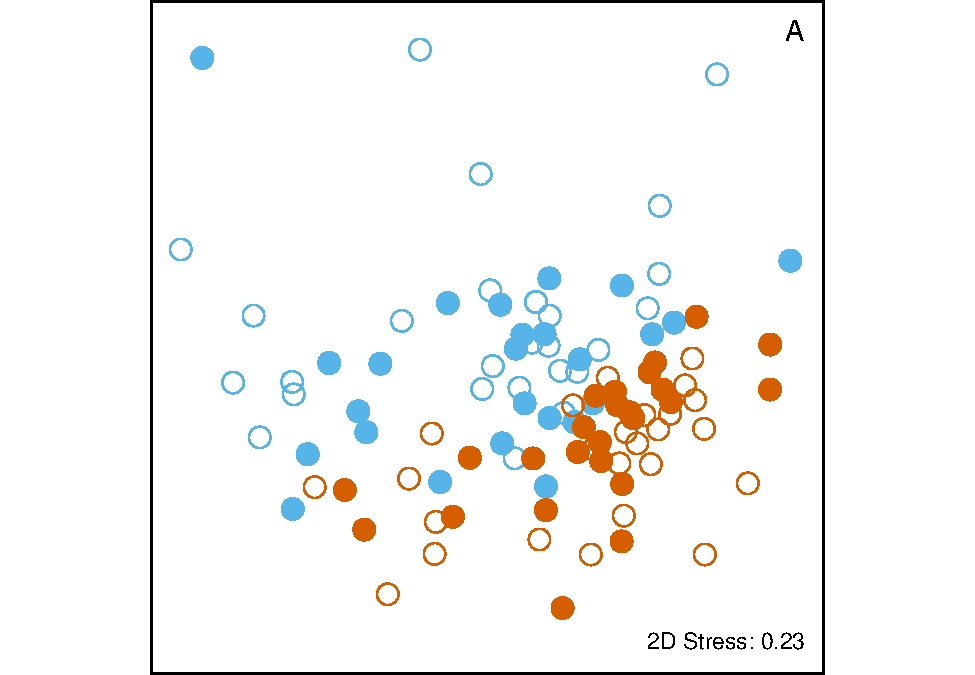
\includegraphics{SealScent_SI_Markdown_2020_1_files/figure-latex/Colony membership in SSB and FWB mom-pup pairs-1.pdf}

\begin{Shaded}
\begin{Highlighting}[]
\NormalTok{## mother-offspring similarity plot}
\CommentTok{# create color palette for the plot}
\NormalTok{clr <-}\StringTok{ }\KeywordTok{c}\NormalTok{(}\StringTok{"#D55E00"}\NormalTok{, }\StringTok{"red"}\NormalTok{, }\StringTok{"#56B4E9"}\NormalTok{, }\StringTok{"#009E73"}\NormalTok{,}\StringTok{"#000000"}\NormalTok{, }\StringTok{"#CC79A7"}\NormalTok{) }

\CommentTok{# assign pch values for plotting}
\NormalTok{shp <-}\StringTok{ }\KeywordTok{c}\NormalTok{(}\DecValTok{0}\NormalTok{,}\DecValTok{1}\NormalTok{,}\DecValTok{2}\NormalTok{,}\DecValTok{7}\NormalTok{,}\DecValTok{10}\NormalTok{,}\DecValTok{5}\NormalTok{,}\DecValTok{6}\NormalTok{,}\DecValTok{18}\NormalTok{,}\DecValTok{16}\NormalTok{,}\DecValTok{17}\NormalTok{,}\DecValTok{15}\NormalTok{) }

\CommentTok{# create unique color-pch pairs}
\NormalTok{color_shape_pairs <-}\StringTok{ }\KeywordTok{crossing}\NormalTok{(clr,shp) }

\CommentTok{# randomly sample 50 unique pairs (sample without replacement)}
\KeywordTok{set.seed}\NormalTok{(}\DecValTok{123}\NormalTok{) }\CommentTok{# always get same pairs in a run}
\NormalTok{color_shape_pairs <-}\StringTok{ }\NormalTok{color_shape_pairs[}\KeywordTok{sample}\NormalTok{(}\KeywordTok{nrow}\NormalTok{(color_shape_pairs), }\DecValTok{50}\NormalTok{),] }

\CommentTok{# assign new dataframes to transform scent_nmds$clr & shp with the unique values we created}
\NormalTok{color_shape_pairs_plot <-}\StringTok{ }\KeywordTok{rbind}\NormalTok{(color_shape_pairs[}\DecValTok{1}\OperatorTok{:}\DecValTok{25}\NormalTok{,],color_shape_pairs[}\DecValTok{1}\OperatorTok{:}\DecValTok{7}\NormalTok{,]}
\NormalTok{                                ,color_shape_pairs[}\DecValTok{7}\NormalTok{,],  color_shape_pairs[}\DecValTok{8}\OperatorTok{:}\DecValTok{25}\NormalTok{,], }
\NormalTok{                                color_shape_pairs[}\DecValTok{26}\OperatorTok{:}\DecValTok{50}\NormalTok{,], color_shape_pairs[}\DecValTok{26}\OperatorTok{:}\DecValTok{50}\NormalTok{,])}
\NormalTok{scent_nmds}\OperatorTok{$}\NormalTok{clr <-}\StringTok{ }\KeywordTok{as.factor}\NormalTok{(color_shape_pairs_plot}\OperatorTok{$}\NormalTok{clr)}
\NormalTok{scent_nmds}\OperatorTok{$}\NormalTok{shp <-}\StringTok{ }\KeywordTok{as.factor}\NormalTok{(color_shape_pairs_plot}\OperatorTok{$}\NormalTok{shp)}

\CommentTok{# call family plot}
\NormalTok{mp_family_gg <-}\StringTok{ }\KeywordTok{ggplot}\NormalTok{(}\DataTypeTok{data =}\NormalTok{ scent_nmds,}\KeywordTok{aes}\NormalTok{(MDS1,MDS2, }\DataTypeTok{color =}\NormalTok{ clr, }\DataTypeTok{shape =}\NormalTok{ shp)) }\OperatorTok{+}\StringTok{ }
\StringTok{  }\KeywordTok{geom_point}\NormalTok{(}\DataTypeTok{size =} \FloatTok{4.5}\NormalTok{) }\OperatorTok{+}
\StringTok{  }\KeywordTok{scale_shape_manual}\NormalTok{(}\DataTypeTok{values =} \KeywordTok{as.numeric}\NormalTok{(}\KeywordTok{levels}\NormalTok{(scent_nmds}\OperatorTok{$}\NormalTok{shp))) }\OperatorTok{+}
\StringTok{  }\KeywordTok{theme_void}\NormalTok{() }\OperatorTok{+}\StringTok{ }
\StringTok{  }\KeywordTok{ylim}\NormalTok{(}\OperatorTok{-}\FloatTok{0.75}\NormalTok{,}\FloatTok{1.1}\NormalTok{) }\OperatorTok{+}
\StringTok{  }\KeywordTok{scale_color_manual}\NormalTok{(}\DataTypeTok{values =} \KeywordTok{levels}\NormalTok{(scent_nmds}\OperatorTok{$}\NormalTok{clr)) }\OperatorTok{+}
\StringTok{  }\KeywordTok{annotate}\NormalTok{(}\StringTok{"text"}\NormalTok{, }\DataTypeTok{x =} \FloatTok{0.64}\NormalTok{, }\DataTypeTok{y =} \FloatTok{1.1}\NormalTok{, }\DataTypeTok{label =} \StringTok{"B"}\NormalTok{, }\DataTypeTok{size =} \DecValTok{5}\NormalTok{) }\OperatorTok{+}
\StringTok{  }\KeywordTok{annotate}\NormalTok{(}\StringTok{"text"}\NormalTok{, }\DataTypeTok{x =} \FloatTok{0.48}\NormalTok{, }\DataTypeTok{y =} \OperatorTok{-}\FloatTok{0.74}\NormalTok{, }\DataTypeTok{label =} \StringTok{"2D Stress: 0.23"}\NormalTok{, }\DataTypeTok{size =} \DecValTok{4}\NormalTok{) }\OperatorTok{+}
\StringTok{  }\KeywordTok{theme}\NormalTok{(}\DataTypeTok{panel.background =} \KeywordTok{element_rect}\NormalTok{(}\DataTypeTok{colour =} \StringTok{"black"}\NormalTok{, }\DataTypeTok{size =} \DecValTok{1}\NormalTok{,}
                                        \DataTypeTok{fill =} \OtherTok{NA}\NormalTok{), }\DataTypeTok{aspect.ratio =} \DecValTok{1}\NormalTok{, }
        \DataTypeTok{legend.position =} \StringTok{"none"}\NormalTok{) }
\NormalTok{mp_family_gg}
\end{Highlighting}
\end{Shaded}

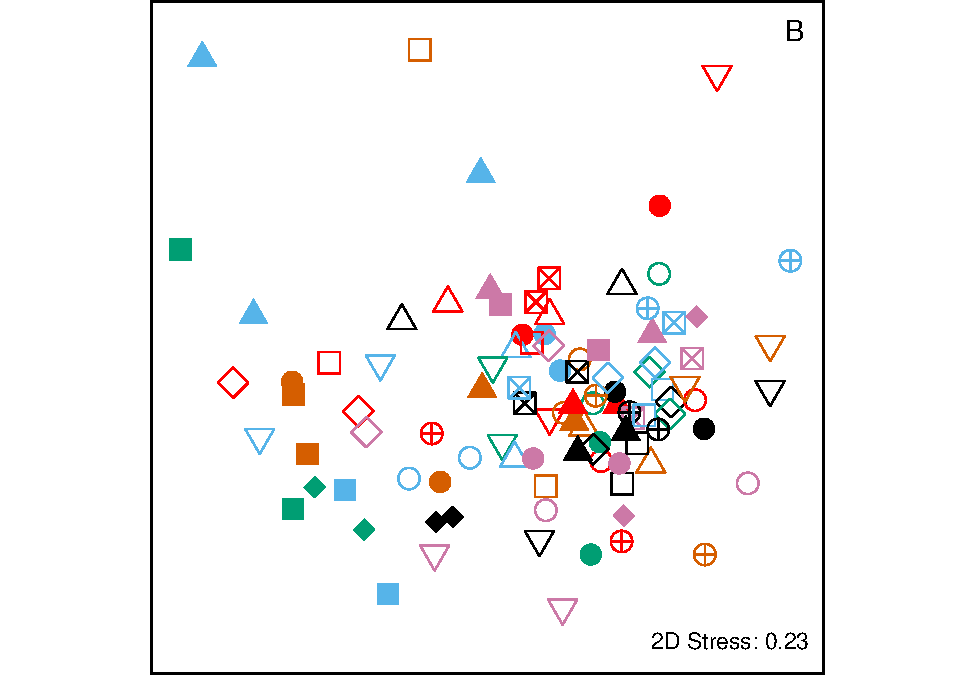
\includegraphics{SealScent_SI_Markdown_2020_1_files/figure-latex/Colony membership in SSB and FWB mom-pup pairs-2.pdf}

\subsection{PERMANOVA for mother-pup similiarity and colony
membership}\label{permanova-for-mother-pup-similiarity-and-colony-membership}

\begin{Shaded}
\begin{Highlighting}[]
\CommentTok{# set seed to reproduce the same outcome (can vary due to different permutations!)}
\KeywordTok{set.seed}\NormalTok{(}\DecValTok{123}\NormalTok{)}

\CommentTok{# set counter for while loop}
\NormalTok{perm_count <-}\StringTok{ }\KeywordTok{c}\NormalTok{(}\DecValTok{99}\NormalTok{)}

\CommentTok{# iterate different significance levels with a while-loop}
\ControlFlowTok{while}\NormalTok{ (perm_count }\OperatorTok{<=}\StringTok{ }\DecValTok{99999}\NormalTok{) \{}\CommentTok{# end while-loop after the run for 99999 permutations}
\NormalTok{  permanova_result_MP <-}\StringTok{ }\KeywordTok{adonis}\NormalTok{(scent }\OperatorTok{~}\StringTok{ }\NormalTok{age}\OperatorTok{+}\NormalTok{colony}\OperatorTok{+}\NormalTok{colony}\OperatorTok{:}\NormalTok{family, }
         \DataTypeTok{data =}\NormalTok{ scent_factors,}
         \DataTypeTok{method =} \StringTok{"bray"}\NormalTok{,}
         \DataTypeTok{permutations =}\NormalTok{ perm_count)}
  \KeywordTok{print}\NormalTok{(permanova_result_MP)}
  
\NormalTok{  perm_count <-}\StringTok{ }\NormalTok{(perm_count}\OperatorTok{*}\DecValTok{10}\NormalTok{)}\OperatorTok{+}\DecValTok{9} \CommentTok{# ends while-iteration after it increases to 999999}
\NormalTok{\}}\CommentTok{#while}
\end{Highlighting}
\end{Shaded}

\begin{verbatim}
## 
## Call:
## adonis(formula = scent ~ age + colony + colony:family, data = scent_factors,      permutations = perm_count, method = "bray") 
## 
## Permutation: free
## Number of permutations: 99
## 
## Terms added sequentially (first to last)
## 
##                Df SumsOfSqs MeanSqs F.Model      R2 Pr(>F)   
## age             1    0.3217 0.32170  2.6896 0.02253   0.02 * 
## colony          1    1.0847 1.08475  9.0692 0.07599   0.01 **
## colony:family   2    1.3870 0.69351  5.7982 0.09716   0.01 **
## Residuals      96   11.4823 0.11961         0.80432          
## Total         100   14.2758                 1.00000          
## ---
## Signif. codes:  0 '***' 0.001 '**' 0.01 '*' 0.05 '.' 0.1 ' ' 1
## 
## Call:
## adonis(formula = scent ~ age + colony + colony:family, data = scent_factors,      permutations = perm_count, method = "bray") 
## 
## Permutation: free
## Number of permutations: 999
## 
## Terms added sequentially (first to last)
## 
##                Df SumsOfSqs MeanSqs F.Model      R2 Pr(>F)    
## age             1    0.3217 0.32170  2.6896 0.02253  0.011 *  
## colony          1    1.0847 1.08475  9.0692 0.07599  0.001 ***
## colony:family   2    1.3870 0.69351  5.7982 0.09716  0.001 ***
## Residuals      96   11.4823 0.11961         0.80432           
## Total         100   14.2758                 1.00000           
## ---
## Signif. codes:  0 '***' 0.001 '**' 0.01 '*' 0.05 '.' 0.1 ' ' 1
## 
## Call:
## adonis(formula = scent ~ age + colony + colony:family, data = scent_factors,      permutations = perm_count, method = "bray") 
## 
## Permutation: free
## Number of permutations: 9999
## 
## Terms added sequentially (first to last)
## 
##                Df SumsOfSqs MeanSqs F.Model      R2 Pr(>F)    
## age             1    0.3217 0.32170  2.6896 0.02253 0.0045 ** 
## colony          1    1.0847 1.08475  9.0692 0.07599 0.0001 ***
## colony:family   2    1.3870 0.69351  5.7982 0.09716 0.0001 ***
## Residuals      96   11.4823 0.11961         0.80432           
## Total         100   14.2758                 1.00000           
## ---
## Signif. codes:  0 '***' 0.001 '**' 0.01 '*' 0.05 '.' 0.1 ' ' 1
## 
## Call:
## adonis(formula = scent ~ age + colony + colony:family, data = scent_factors,      permutations = perm_count, method = "bray") 
## 
## Permutation: free
## Number of permutations: 99999
## 
## Terms added sequentially (first to last)
## 
##                Df SumsOfSqs MeanSqs F.Model      R2  Pr(>F)    
## age             1    0.3217 0.32170  2.6896 0.02253 0.00403 ** 
## colony          1    1.0847 1.08475  9.0692 0.07599   1e-05 ***
## colony:family   2    1.3870 0.69351  5.7982 0.09716   1e-05 ***
## Residuals      96   11.4823 0.11961         0.80432            
## Total         100   14.2758                 1.00000            
## ---
## Signif. codes:  0 '***' 0.001 '**' 0.01 '*' 0.05 '.' 0.1 ' ' 1
\end{verbatim}

Post-hoc betadisper and pairwise comparisons for mother-pup pair
PERMANOVA results

\begin{Shaded}
\begin{Highlighting}[]
\CommentTok{# test for group dispersal}
\CommentTok{# for different colonies}
\NormalTok{mod_colony  <-}\StringTok{ }\KeywordTok{betadisper}\NormalTok{(}\KeywordTok{vegdist}\NormalTok{(scent), scent_factors}\OperatorTok{$}\NormalTok{colony, }\DataTypeTok{type =} \StringTok{"median"}\NormalTok{)}
\KeywordTok{anova}\NormalTok{(mod_colony)}
\end{Highlighting}
\end{Shaded}

\begin{verbatim}
## Analysis of Variance Table
## 
## Response: Distances
##           Df Sum Sq  Mean Sq F value  Pr(>F)  
## Groups     1 0.0442 0.044201   5.136 0.02561 *
## Residuals 99 0.8520 0.008606                  
## ---
## Signif. codes:  0 '***' 0.001 '**' 0.01 '*' 0.05 '.' 0.1 ' ' 1
\end{verbatim}

\begin{Shaded}
\begin{Highlighting}[]
\CommentTok{# for different ages (mom vs pup)}
\NormalTok{mod_age <-}\StringTok{ }\KeywordTok{betadisper}\NormalTok{(}\KeywordTok{vegdist}\NormalTok{(scent), scent_factors}\OperatorTok{$}\NormalTok{age, }\DataTypeTok{type =} \StringTok{"median"}\NormalTok{)}
\KeywordTok{anova}\NormalTok{(mod_age)}
\end{Highlighting}
\end{Shaded}

\begin{verbatim}
## Analysis of Variance Table
## 
## Response: Distances
##           Df  Sum Sq   Mean Sq F value Pr(>F)
## Groups     1 0.01305 0.0130477  1.4726 0.2278
## Residuals 99 0.87718 0.0088604
\end{verbatim}

\begin{Shaded}
\begin{Highlighting}[]
\CommentTok{# for different combinations of age and colony identity}
\NormalTok{mod_BeachAge <-}\StringTok{ }\KeywordTok{betadisper}\NormalTok{(}\KeywordTok{vegdist}\NormalTok{(scent), scent_nmds}\OperatorTok{$}\NormalTok{BeachAge, }\DataTypeTok{type =} \StringTok{"median"}\NormalTok{)}
\KeywordTok{anova}\NormalTok{(mod_BeachAge)}
\end{Highlighting}
\end{Shaded}

\begin{verbatim}
## Analysis of Variance Table
## 
## Response: Distances
##           Df  Sum Sq   Mean Sq F value Pr(>F)
## Groups     3 0.04845 0.0161488  1.9067 0.1336
## Residuals 97 0.82153 0.0084694
\end{verbatim}

Pairwise comparison between all possible combinations of mother-pup
pairs based on colony identity and age

\begin{Shaded}
\begin{Highlighting}[]
\KeywordTok{set.seed}\NormalTok{(}\DecValTok{123}\NormalTok{) }\CommentTok{# for comparability as results do not change when compared to manuscript}
\NormalTok{pairwiseAdonis}\OperatorTok{::}\KeywordTok{pairwise.adonis}\NormalTok{(scent, scent_nmds}\OperatorTok{$}\NormalTok{BeachAge, }\DataTypeTok{perm =} \DecValTok{99999}\NormalTok{)}
\end{Highlighting}
\end{Shaded}

\begin{verbatim}
##            pairs Df SumsOfSqs  F.Model         R2 p.value p.adjusted sig
## 1 SSB_1 vs SSB_2  1 0.3515433 2.415725 0.04698416 0.01227    0.07362    
## 2 SSB_1 vs FWB_1  1 0.5291662 4.272400 0.08173337 0.00004    0.00024  **
## 3 SSB_1 vs FWB_2  1 0.5542266 4.218847 0.08079165 0.00003    0.00018  **
## 4 SSB_2 vs FWB_1  1 0.8481620 6.618475 0.11899778 0.00001    0.00006 ***
## 5 SSB_2 vs FWB_2  1 0.8397841 6.197227 0.11227424 0.00001    0.00006 ***
## 6 FWB_1 vs FWB_2  1 0.2514355 2.212658 0.04406574 0.01906    0.11436
\end{verbatim}

\begin{Shaded}
\begin{Highlighting}[]
\CommentTok{# Pairwise group dispersal tests}

\CommentTok{# scent, scent_factors and scent_nmds are all data.frames the have the same row setup.}
\CommentTok{# Meaning: Each row respresenting an individual is identical in each data.frame.}
\CommentTok{# Thus, we can index pairs based on scent_nmds$BeachAge manually.}

\NormalTok{pairwise_betadisper1 <-}\StringTok{ }\KeywordTok{betadisper}\NormalTok{(}\KeywordTok{vegdist}\NormalTok{(scent[scent_nmds}\OperatorTok{$}\NormalTok{BeachAge }\OperatorTok{==}\StringTok{ "SSB_1"} \OperatorTok{|}\StringTok{ }\NormalTok{scent_nmds}\OperatorTok{$}\NormalTok{BeachAge }\OperatorTok{==}\StringTok{ "SSB_2"}\NormalTok{,]), }
\NormalTok{                            scent_nmds}\OperatorTok{$}\NormalTok{BeachAge[scent_nmds}\OperatorTok{$}\NormalTok{BeachAge }\OperatorTok{==}\StringTok{ "SSB_1"} \OperatorTok{|}\StringTok{ }\NormalTok{scent_nmds}\OperatorTok{$}\NormalTok{BeachAge }\OperatorTok{==}\StringTok{ "SSB_2"}\NormalTok{],}
                            \DataTypeTok{type =} \StringTok{"median"}\NormalTok{)}
\KeywordTok{anova}\NormalTok{(pairwise_betadisper1)}
\end{Highlighting}
\end{Shaded}

\begin{verbatim}
## Analysis of Variance Table
## 
## Response: Distances
##           Df  Sum Sq   Mean Sq F value Pr(>F)
## Groups     1 0.00104 0.0010419  0.1024 0.7504
## Residuals 49 0.49872 0.0101780
\end{verbatim}

\begin{Shaded}
\begin{Highlighting}[]
\NormalTok{pairwise_betadisper2 <-}\StringTok{ }\KeywordTok{betadisper}\NormalTok{(}\KeywordTok{vegdist}\NormalTok{(scent[scent_nmds}\OperatorTok{$}\NormalTok{BeachAge }\OperatorTok{==}\StringTok{ "SSB_1"} \OperatorTok{|}\StringTok{ }\NormalTok{scent_nmds}\OperatorTok{$}\NormalTok{BeachAge }\OperatorTok{==}\StringTok{ "FWB_1"}\NormalTok{,]), }
\NormalTok{                            scent_nmds}\OperatorTok{$}\NormalTok{BeachAge[scent_nmds}\OperatorTok{$}\NormalTok{BeachAge }\OperatorTok{==}\StringTok{ "SSB_1"} \OperatorTok{|}\StringTok{ }\NormalTok{scent_nmds}\OperatorTok{$}\NormalTok{BeachAge }\OperatorTok{==}\StringTok{ "FWB_1"}\NormalTok{],}
                            \DataTypeTok{type =} \StringTok{"median"}\NormalTok{)}
\KeywordTok{anova}\NormalTok{(pairwise_betadisper2)}
\end{Highlighting}
\end{Shaded}

\begin{verbatim}
## Analysis of Variance Table
## 
## Response: Distances
##           Df  Sum Sq   Mean Sq F value  Pr(>F)  
## Groups     1 0.02731 0.0273093  3.5184 0.06678 .
## Residuals 48 0.37256 0.0077618                  
## ---
## Signif. codes:  0 '***' 0.001 '**' 0.01 '*' 0.05 '.' 0.1 ' ' 1
\end{verbatim}

\begin{Shaded}
\begin{Highlighting}[]
\NormalTok{pairwise_betadisper3 <-}\StringTok{ }\KeywordTok{betadisper}\NormalTok{(}\KeywordTok{vegdist}\NormalTok{(scent[scent_nmds}\OperatorTok{$}\NormalTok{BeachAge }\OperatorTok{==}\StringTok{ "SSB_1"} \OperatorTok{|}\StringTok{ }\NormalTok{scent_nmds}\OperatorTok{$}\NormalTok{BeachAge }\OperatorTok{==}\StringTok{ "FWB_2"}\NormalTok{,]), }
\NormalTok{                            scent_nmds}\OperatorTok{$}\NormalTok{BeachAge[scent_nmds}\OperatorTok{$}\NormalTok{BeachAge }\OperatorTok{==}\StringTok{ "SSB_1"} \OperatorTok{|}\StringTok{ }\NormalTok{scent_nmds}\OperatorTok{$}\NormalTok{BeachAge }\OperatorTok{==}\StringTok{ "FWB_2"}\NormalTok{],}
                            \DataTypeTok{type =} \StringTok{"median"}\NormalTok{)}
\KeywordTok{anova}\NormalTok{(pairwise_betadisper3)}
\end{Highlighting}
\end{Shaded}

\begin{verbatim}
## Analysis of Variance Table
## 
## Response: Distances
##           Df  Sum Sq   Mean Sq F value Pr(>F)
## Groups     1 0.00796 0.0079639  0.9519 0.3341
## Residuals 48 0.40159 0.0083665
\end{verbatim}

\begin{Shaded}
\begin{Highlighting}[]
\NormalTok{pairwise_betadisper4 <-}\StringTok{ }\KeywordTok{betadisper}\NormalTok{(}\KeywordTok{vegdist}\NormalTok{(scent[scent_nmds}\OperatorTok{$}\NormalTok{BeachAge }\OperatorTok{==}\StringTok{ "SSB_2"} \OperatorTok{|}\StringTok{ }\NormalTok{scent_nmds}\OperatorTok{$}\NormalTok{BeachAge }\OperatorTok{==}\StringTok{ "FWB_1"}\NormalTok{,]), }
\NormalTok{                            scent_nmds}\OperatorTok{$}\NormalTok{BeachAge[scent_nmds}\OperatorTok{$}\NormalTok{BeachAge }\OperatorTok{==}\StringTok{ "SSB_2"} \OperatorTok{|}\StringTok{ }\NormalTok{scent_nmds}\OperatorTok{$}\NormalTok{BeachAge }\OperatorTok{==}\StringTok{ "FWB_1"}\NormalTok{],}
                            \DataTypeTok{type =} \StringTok{"median"}\NormalTok{)}
\KeywordTok{anova}\NormalTok{(pairwise_betadisper4)}
\end{Highlighting}
\end{Shaded}

\begin{verbatim}
## Analysis of Variance Table
## 
## Response: Distances
##           Df  Sum Sq  Mean Sq F value  Pr(>F)  
## Groups     1 0.03973 0.039734  4.5784 0.03738 *
## Residuals 49 0.42525 0.008679                  
## ---
## Signif. codes:  0 '***' 0.001 '**' 0.01 '*' 0.05 '.' 0.1 ' ' 1
\end{verbatim}

\begin{Shaded}
\begin{Highlighting}[]
\NormalTok{pairwise_betadisper5 <-}\StringTok{ }\KeywordTok{betadisper}\NormalTok{(}\KeywordTok{vegdist}\NormalTok{(scent[scent_nmds}\OperatorTok{$}\NormalTok{BeachAge }\OperatorTok{==}\StringTok{ "SSB_2"} \OperatorTok{|}\StringTok{ }\NormalTok{scent_nmds}\OperatorTok{$}\NormalTok{BeachAge }\OperatorTok{==}\StringTok{ "FWB_2"}\NormalTok{,]), }
\NormalTok{                            scent_nmds}\OperatorTok{$}\NormalTok{BeachAge[scent_nmds}\OperatorTok{$}\NormalTok{BeachAge }\OperatorTok{==}\StringTok{ "SSB_2"} \OperatorTok{|}\StringTok{ }\NormalTok{scent_nmds}\OperatorTok{$}\NormalTok{BeachAge }\OperatorTok{==}\StringTok{ "FWB_2"}\NormalTok{],}
                            \DataTypeTok{type =} \StringTok{"median"}\NormalTok{)}
\KeywordTok{anova}\NormalTok{(pairwise_betadisper5)}
\end{Highlighting}
\end{Shaded}

\begin{verbatim}
## Analysis of Variance Table
## 
## Response: Distances
##           Df  Sum Sq  Mean Sq F value Pr(>F)
## Groups     1 0.01502 0.015016  1.6302 0.2077
## Residuals 49 0.45134 0.009211
\end{verbatim}

\begin{Shaded}
\begin{Highlighting}[]
\NormalTok{pairwise_betadisper6 <-}\StringTok{ }\KeywordTok{betadisper}\NormalTok{(}\KeywordTok{vegdist}\NormalTok{(scent[scent_nmds}\OperatorTok{$}\NormalTok{BeachAge }\OperatorTok{==}\StringTok{ "FWB_1"} \OperatorTok{|}\StringTok{ }\NormalTok{scent_nmds}\OperatorTok{$}\NormalTok{BeachAge }\OperatorTok{==}\StringTok{ "FWB_2"}\NormalTok{,]), }
\NormalTok{                            scent_nmds}\OperatorTok{$}\NormalTok{BeachAge[scent_nmds}\OperatorTok{$}\NormalTok{BeachAge }\OperatorTok{==}\StringTok{ "FWB_1"} \OperatorTok{|}\StringTok{ }\NormalTok{scent_nmds}\OperatorTok{$}\NormalTok{BeachAge }\OperatorTok{==}\StringTok{ "FWB_2"}\NormalTok{],}
                            \DataTypeTok{type =} \StringTok{"median"}\NormalTok{)}
\KeywordTok{anova}\NormalTok{(pairwise_betadisper6)}
\end{Highlighting}
\end{Shaded}

\begin{verbatim}
## Analysis of Variance Table
## 
## Response: Distances
##           Df  Sum Sq   Mean Sq F value Pr(>F)
## Groups     1 0.00579 0.0057933  0.8476 0.3618
## Residuals 48 0.32807 0.0068347
\end{verbatim}

\subsection{NMDS scaling and colony membership in six pup
colonies}\label{nmds-scaling-and-colony-membership-in-six-pup-colonies}

\begin{Shaded}
\begin{Highlighting}[]
\KeywordTok{load}\NormalTok{(}\StringTok{"RData/objects/pup_colonies_alignment_GCalignR.RData"}\NormalTok{)}
\NormalTok{scent_factors_raw <-}\StringTok{ }\KeywordTok{read_delim}\NormalTok{(}\StringTok{"documents/metadata_seal_scent.txt"}\NormalTok{, }
                                \StringTok{"}\CharTok{\textbackslash{}t}\StringTok{"}\NormalTok{, }\DataTypeTok{escape_double =} \OtherTok{FALSE}\NormalTok{, }\DataTypeTok{trim_ws =} \OtherTok{TRUE}\NormalTok{)}
\NormalTok{scent_factors_raw <-}\StringTok{ }\KeywordTok{as.data.frame}\NormalTok{(scent_factors_raw[}\OperatorTok{-}\KeywordTok{c}\NormalTok{(}\DecValTok{194}\OperatorTok{:}\DecValTok{209}\NormalTok{),])}

\CommentTok{# set sample names as row names, ensure there are no duplicates}
\NormalTok{scent_factors <-}\StringTok{ }\NormalTok{scent_factors_raw[,}\OperatorTok{-}\DecValTok{1}\NormalTok{]}
\KeywordTok{rownames}\NormalTok{(scent_factors) <-}\StringTok{ }\NormalTok{scent_factors_raw[,}\DecValTok{1}\NormalTok{]}

\NormalTok{## check for empty samples, i.e. no peaks}
\NormalTok{x <-}\StringTok{ }\KeywordTok{apply}\NormalTok{(pup_colonies_aligned}\OperatorTok{$}\NormalTok{aligned}\OperatorTok{$}\NormalTok{RT, }\DecValTok{2}\NormalTok{, sum)}
\NormalTok{x <-}\StringTok{ }\KeywordTok{which}\NormalTok{(x }\OperatorTok{==}\StringTok{ }\DecValTok{0}\NormalTok{)}

\NormalTok{## normalise area and return a data frame}
\NormalTok{scent <-}\StringTok{ }\KeywordTok{norm_peaks}\NormalTok{(pup_colonies_aligned, }\DataTypeTok{conc_col_name =} \StringTok{"Area"}\NormalTok{,}\DataTypeTok{rt_col_name =} \StringTok{"RT"}\NormalTok{,}
                    \DataTypeTok{out =} \StringTok{"data.frame"}\NormalTok{) }
\NormalTok{## common transformation for abundance data to reduce the extent of mean-variance trends}
\NormalTok{scent <-}\StringTok{ }\KeywordTok{log}\NormalTok{(scent }\OperatorTok{+}\StringTok{ }\DecValTok{1}\NormalTok{) }

\NormalTok{## subset scent_factors}
\NormalTok{scent_factors <-}\StringTok{ }\NormalTok{scent_factors[}\KeywordTok{rownames}\NormalTok{(scent_factors) }\OperatorTok\StringTok{ }\KeywordTok{rownames}\NormalTok{(scent),]}
\NormalTok{scent <-}\StringTok{ }\NormalTok{scent[}\KeywordTok{rownames}\NormalTok{(scent) }\OperatorTok\StringTok{ }\KeywordTok{rownames}\NormalTok{(scent_factors),]}

\NormalTok{## keep order of rows consistent}
\NormalTok{scent <-}\StringTok{ }\NormalTok{scent[}\KeywordTok{match}\NormalTok{(}\KeywordTok{rownames}\NormalTok{(scent_factors),}\KeywordTok{rownames}\NormalTok{(scent)),] }

\NormalTok{## get number of compounds for each individual sample after alignment}
\NormalTok{num_comp <-}\StringTok{ }\KeywordTok{as.vector}\NormalTok{(}\KeywordTok{apply}\NormalTok{(scent, }\DecValTok{1}\NormalTok{, }\ControlFlowTok{function}\NormalTok{(x) }\KeywordTok{length}\NormalTok{(x[x}\OperatorTok{>}\DecValTok{0}\NormalTok{])))}

\NormalTok{## bray-curtis similarity}
\NormalTok{scent_nmds.obj <-}\StringTok{ }\KeywordTok{metaMDS}\NormalTok{(}\DataTypeTok{comm =}\NormalTok{ scent, }\DataTypeTok{k =} \DecValTok{2}\NormalTok{, }\DataTypeTok{try =} \DecValTok{999}\NormalTok{, }
                          \DataTypeTok{trymax =} \DecValTok{9999}\NormalTok{, }\DataTypeTok{distance =} \StringTok{"bray"}\NormalTok{) }
\NormalTok{## MDS outcome evaluated with PCA for factor colony in metadata table for individuals}
\NormalTok{scent_nmds <-}\StringTok{ }\KeywordTok{with}\NormalTok{(scent_factors, }\KeywordTok{MDSrotate}\NormalTok{(scent_nmds.obj, colony))}

\NormalTok{## get x and y coordinates}
\NormalTok{scent_nmds <-}\StringTok{ }\KeywordTok{as.data.frame}\NormalTok{(scent_nmds[[}\StringTok{"points"}\NormalTok{]])  }

\NormalTok{## add the colony as a factor to each sample}
\NormalTok{scent_nmds <-}\StringTok{ }\KeywordTok{cbind}\NormalTok{(scent_nmds,}
                    \DataTypeTok{age =}\NormalTok{ scent_factors[[}\StringTok{"age"}\NormalTok{]],}
                    \DataTypeTok{tissue_tag =}\NormalTok{ scent_factors[[}\StringTok{"tissue_tag"}\NormalTok{]],}
                    \DataTypeTok{colony =}\NormalTok{ scent_factors[[}\StringTok{"colony"}\NormalTok{]],}
                    \DataTypeTok{family =} \KeywordTok{as.factor}\NormalTok{(scent_factors[[}\StringTok{"family"}\NormalTok{]]),}
                    \DataTypeTok{clr =} \KeywordTok{as.factor}\NormalTok{(scent_factors[[}\StringTok{"clr"}\NormalTok{]]),}
                    \DataTypeTok{shp =} \KeywordTok{as.factor}\NormalTok{(scent_factors[[}\StringTok{"shp"}\NormalTok{]]),}
                    \DataTypeTok{gcms =} \KeywordTok{as.factor}\NormalTok{(scent_factors[[}\StringTok{"gcms_run"}\NormalTok{]]),}
                    \DataTypeTok{peak_res =} \KeywordTok{as.factor}\NormalTok{(scent_factors[[}\StringTok{"peak_res"}\NormalTok{]]),}
                    \DataTypeTok{sample_qlty =} \KeywordTok{as.factor}\NormalTok{(scent_factors[[}\StringTok{"sample_qlty"}\NormalTok{]]),}
                    \DataTypeTok{vialdate =} \KeywordTok{as.factor}\NormalTok{(scent_factors[[}\StringTok{"gcms_vialdate"}\NormalTok{]]),}
                    \DataTypeTok{captured =} \KeywordTok{as.factor}\NormalTok{(scent_factors[[}\StringTok{"capture_date"}\NormalTok{]]),}
                    \DataTypeTok{sex =}\NormalTok{ scent_factors[[}\StringTok{"sex"}\NormalTok{]],}
                    \DataTypeTok{num_comp =}\NormalTok{ num_comp)}
\CommentTok{# creates & adds new variable BeachAge }
\NormalTok{scent_nmds <-}\StringTok{ }\NormalTok{scent_nmds }\OperatorTok\StringTok{ }\KeywordTok{mutate}\NormalTok{(}\DataTypeTok{BeachAge =} \KeywordTok{str_c}\NormalTok{(colony, age, }\DataTypeTok{sep =} \StringTok{"_"}\NormalTok{)) }
\end{Highlighting}
\end{Shaded}

Colony membership plot for six pup colonies (Supplementary figure)

\begin{Shaded}
\begin{Highlighting}[]
\KeywordTok{load}\NormalTok{(}\StringTok{"RData/objects/pup_colonies_nmds_scaling.RData"}\NormalTok{)}

\NormalTok{pup_colony_gg <-}\StringTok{ }\KeywordTok{ggplot}\NormalTok{(}\DataTypeTok{data =}\NormalTok{ scent_nmds, }\KeywordTok{aes}\NormalTok{(MDS1, MDS2, }\DataTypeTok{color =}\NormalTok{ colony, }\DataTypeTok{shape =}\NormalTok{ colony)) }\OperatorTok{+}\StringTok{ }
\StringTok{  }\KeywordTok{geom_point}\NormalTok{(}\DataTypeTok{size =} \FloatTok{4.5}\NormalTok{) }\OperatorTok{+}\StringTok{ }
\StringTok{  }\KeywordTok{scale_shape_manual}\NormalTok{(}\DataTypeTok{values =} \KeywordTok{c}\NormalTok{(}\DecValTok{15}\NormalTok{,}\DecValTok{20}\NormalTok{,}\DecValTok{17}\NormalTok{,}\DecValTok{15}\NormalTok{,}\DecValTok{17}\NormalTok{,}\DecValTok{18}\NormalTok{),}
                     \DataTypeTok{labels =} \KeywordTok{c}\NormalTok{(}\StringTok{"FWB"}\NormalTok{, }\StringTok{"Johnson cove"}\NormalTok{, }\StringTok{"Landing beach"}\NormalTok{, }\StringTok{"Main bay"}\NormalTok{, }\StringTok{"Natural arch"}\NormalTok{, }\StringTok{"SSB"}\NormalTok{)) }\OperatorTok{+}
\StringTok{  }\KeywordTok{scale_color_manual}\NormalTok{(}\DataTypeTok{values =} \KeywordTok{c}\NormalTok{(}\StringTok{"#D55E00"}\NormalTok{, }\StringTok{"#000000"}\NormalTok{, }\StringTok{"#E69F00"}\NormalTok{, }\StringTok{"#009E73"}\NormalTok{, }\StringTok{"#CC79A7"}\NormalTok{, }\StringTok{"#0072B2"}\NormalTok{),}
                     \DataTypeTok{labels =} \KeywordTok{c}\NormalTok{(}\StringTok{"FWB"}\NormalTok{, }\StringTok{"Johnson cove"}\NormalTok{, }\StringTok{"Landing beach"}\NormalTok{, }\StringTok{"Main bay"}\NormalTok{, }\StringTok{"Natural arch"}\NormalTok{, }\StringTok{"SSB"}\NormalTok{)) }\OperatorTok{+}
\StringTok{  }\KeywordTok{theme_void}\NormalTok{() }\OperatorTok{+}\StringTok{ }
\StringTok{  }\KeywordTok{annotate}\NormalTok{(}\StringTok{"text"}\NormalTok{, }\DataTypeTok{x =} \FloatTok{0.6}\NormalTok{, }\DataTypeTok{y =} \OperatorTok{-}\FloatTok{0.94}\NormalTok{, }\DataTypeTok{label =} \StringTok{"2D Stress: 0.24"}\NormalTok{, }\DataTypeTok{size =} \DecValTok{4}\NormalTok{) }\OperatorTok{+}
\StringTok{  }\KeywordTok{theme}\NormalTok{(}\DataTypeTok{panel.background =} \KeywordTok{element_rect}\NormalTok{(}\DataTypeTok{colour =} \StringTok{"black"}\NormalTok{, }\DataTypeTok{size =} \DecValTok{1}\NormalTok{, }\DataTypeTok{fill =} \OtherTok{NA}\NormalTok{),}
        \DataTypeTok{aspect.ratio =} \DecValTok{1}\NormalTok{,}
        \DataTypeTok{legend.position =} \StringTok{"right"}\NormalTok{, }\CommentTok{#c(0.1,0.87),}
        \DataTypeTok{legend.title =} \KeywordTok{element_blank}\NormalTok{(),}
        \CommentTok{# legend.key.size = unit(0.5, "cm"),}
        \CommentTok{# legend.key.width = unit(0.5, "cm"),}
        \DataTypeTok{legend.background =} \KeywordTok{element_rect}\NormalTok{(}\DataTypeTok{size =} \FloatTok{0.3}\NormalTok{, }\DataTypeTok{linetype =} \StringTok{"solid"}\NormalTok{, }\DataTypeTok{color =} \StringTok{"black"}\NormalTok{))}

\NormalTok{pup_colony_gg}
\end{Highlighting}
\end{Shaded}

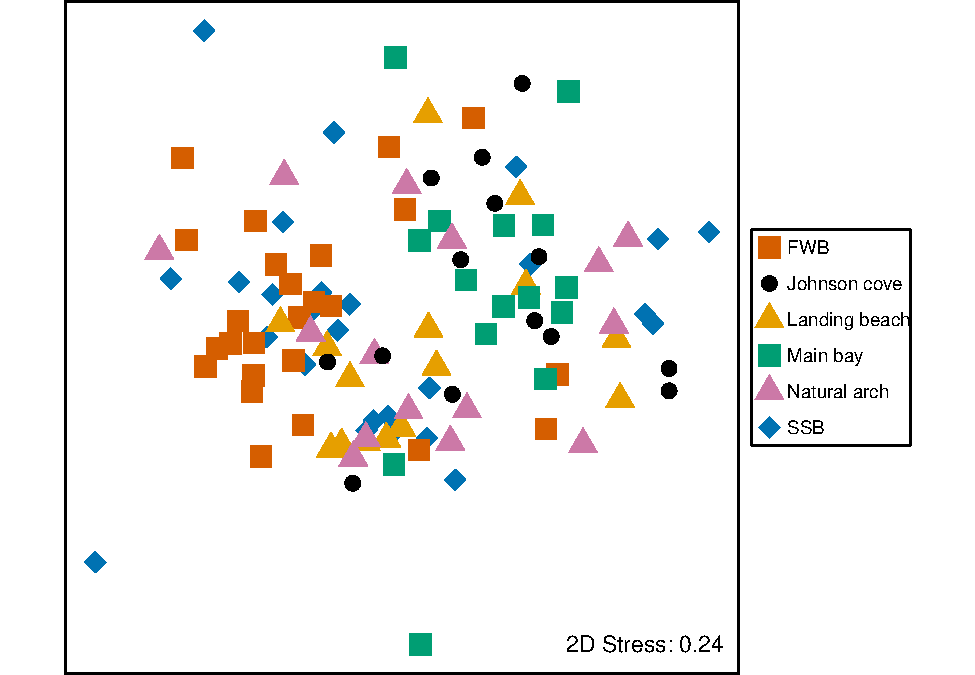
\includegraphics{SealScent_SI_Markdown_2020_1_files/figure-latex/unnamed-chunk-5-1.pdf}

PERMANOVA for colony membership in six pup colonies

\begin{Shaded}
\begin{Highlighting}[]
\CommentTok{# set seed to reproduce the same outcome (can vary due to different permutations!)}
\KeywordTok{set.seed}\NormalTok{(}\DecValTok{123}\NormalTok{)}

\CommentTok{# set counter for while loop}
\NormalTok{perm_count <-}\StringTok{ }\KeywordTok{c}\NormalTok{(}\DecValTok{99}\NormalTok{)}

\CommentTok{# iterate different significance levels with a while-loop}
\ControlFlowTok{while}\NormalTok{ (perm_count }\OperatorTok{<=}\StringTok{ }\DecValTok{99999}\NormalTok{) \{}\CommentTok{# end while-loop after the run for 99999 permutations}
\NormalTok{  permanova_result_pupcols <-}\StringTok{ }\KeywordTok{adonis}\NormalTok{(scent }\OperatorTok{~}\StringTok{ }\NormalTok{age}\OperatorTok{+}\NormalTok{colony}\OperatorTok{+}\NormalTok{colony}\OperatorTok{:}\NormalTok{family, }
         \DataTypeTok{data =}\NormalTok{ scent_factors,}
         \DataTypeTok{method =} \StringTok{"bray"}\NormalTok{,}
         \DataTypeTok{permutations =}\NormalTok{ perm_count)}
  \KeywordTok{print}\NormalTok{(permanova_result_pupcols)}
  
\NormalTok{  perm_count <-}\StringTok{ }\NormalTok{(perm_count}\OperatorTok{*}\DecValTok{10}\NormalTok{)}\OperatorTok{+}\DecValTok{9} \CommentTok{# ends while-iteration after it increases to 999999}
\NormalTok{\}}\CommentTok{#while }
\end{Highlighting}
\end{Shaded}

\begin{verbatim}
## 
## Call:
## adonis(formula = scent ~ age + colony + colony:family, data = scent_factors,      permutations = perm_count, method = "bray") 
## 
## Permutation: free
## Number of permutations: 99
## 
## Terms added sequentially (first to last)
## 
##                Df SumsOfSqs MeanSqs F.Model      R2 Pr(>F)   
## colony          5    3.1874 0.63749  5.1748 0.19128   0.01 **
## colony:family   6    1.4037 0.23395  1.8991 0.08424   0.01 **
## Residuals      98   12.0727 0.12319         0.72449          
## Total         109   16.6639                 1.00000          
## ---
## Signif. codes:  0 '***' 0.001 '**' 0.01 '*' 0.05 '.' 0.1 ' ' 1
## 
## Call:
## adonis(formula = scent ~ age + colony + colony:family, data = scent_factors,      permutations = perm_count, method = "bray") 
## 
## Permutation: free
## Number of permutations: 999
## 
## Terms added sequentially (first to last)
## 
##                Df SumsOfSqs MeanSqs F.Model      R2 Pr(>F)    
## colony          5    3.1874 0.63749  5.1748 0.19128  0.001 ***
## colony:family   6    1.4037 0.23395  1.8991 0.08424  0.001 ***
## Residuals      98   12.0727 0.12319         0.72449           
## Total         109   16.6639                 1.00000           
## ---
## Signif. codes:  0 '***' 0.001 '**' 0.01 '*' 0.05 '.' 0.1 ' ' 1
## 
## Call:
## adonis(formula = scent ~ age + colony + colony:family, data = scent_factors,      permutations = perm_count, method = "bray") 
## 
## Permutation: free
## Number of permutations: 9999
## 
## Terms added sequentially (first to last)
## 
##                Df SumsOfSqs MeanSqs F.Model      R2 Pr(>F)    
## colony          5    3.1874 0.63749  5.1748 0.19128  1e-04 ***
## colony:family   6    1.4037 0.23395  1.8991 0.08424  2e-04 ***
## Residuals      98   12.0727 0.12319         0.72449           
## Total         109   16.6639                 1.00000           
## ---
## Signif. codes:  0 '***' 0.001 '**' 0.01 '*' 0.05 '.' 0.1 ' ' 1
## 
## Call:
## adonis(formula = scent ~ age + colony + colony:family, data = scent_factors,      permutations = perm_count, method = "bray") 
## 
## Permutation: free
## Number of permutations: 99999
## 
## Terms added sequentially (first to last)
## 
##                Df SumsOfSqs MeanSqs F.Model      R2 Pr(>F)    
## colony          5    3.1874 0.63749  5.1748 0.19128  1e-05 ***
## colony:family   6    1.4037 0.23395  1.8991 0.08424  6e-05 ***
## Residuals      98   12.0727 0.12319         0.72449           
## Total         109   16.6639                 1.00000           
## ---
## Signif. codes:  0 '***' 0.001 '**' 0.01 '*' 0.05 '.' 0.1 ' ' 1
\end{verbatim}

Post-hoc tests for PERMANOVA results for six pup colonies

\begin{Shaded}
\begin{Highlighting}[]
\CommentTok{# pairwise PERMANOVA}
\NormalTok{pairwiseAdonis}\OperatorTok{::}\KeywordTok{pairwise.adonis}\NormalTok{(scent, scent_factors}\OperatorTok{$}\NormalTok{colony, }\DataTypeTok{perm =} \DecValTok{99999}\NormalTok{)}
\end{Highlighting}
\end{Shaded}

\begin{verbatim}
##                            pairs Df SumsOfSqs  F.Model         R2 p.value
## 1                     SSB vs FWB  1 0.8086332 6.080018 0.11038519 0.00001
## 2           SSB vs landing_beach  1 0.4880064 3.544865 0.08332062 0.00083
## 3                SSB vs main_bay  1 0.8584284 6.181387 0.13681269 0.00001
## 4            SSB vs natural_arch  1 0.5667911 4.172853 0.09665456 0.00010
## 5                 SSB vs johnson  1 0.6168108 4.407128 0.10392422 0.00005
## 6           FWB vs landing_beach  1 0.5117674 4.168468 0.09885273 0.00009
## 7                FWB vs main_bay  1 0.9039828 7.289582 0.16095494 0.00001
## 8            FWB vs natural_arch  1 0.9556981 7.905832 0.17221847 0.00001
## 9                 FWB vs johnson  1 0.8911846 7.145352 0.16185966 0.00001
## 10     landing_beach vs main_bay  1 0.4229462 3.322412 0.10607138 0.00186
## 11 landing_beach vs natural_arch  1 0.3694950 3.002564 0.09684889 0.00413
## 12      landing_beach vs johnson  1 0.3459312 2.694198 0.09073145 0.01225
## 13      main_bay vs natural_arch  1 0.7381617 5.917530 0.17446818 0.00001
## 14           main_bay vs johnson  1 0.4083747 3.137902 0.10411813 0.00024
## 15       natural_arch vs johnson  1 0.3053377 2.428242 0.08251399 0.01651
##    p.adjusted sig
## 1     0.00015  **
## 2     0.01245   .
## 3     0.00015  **
## 4     0.00150   *
## 5     0.00075  **
## 6     0.00135   *
## 7     0.00015  **
## 8     0.00015  **
## 9     0.00015  **
## 10    0.02790   .
## 11    0.06195    
## 12    0.18375    
## 13    0.00015  **
## 14    0.00360   *
## 15    0.24765
\end{verbatim}

\begin{Shaded}
\begin{Highlighting}[]
\CommentTok{# test for group dispersal}
\NormalTok{mod2 <-}\StringTok{ }\KeywordTok{betadisper}\NormalTok{(}\KeywordTok{vegdist}\NormalTok{(scent), scent_factors}\OperatorTok{$}\NormalTok{colony, }\DataTypeTok{type =} \StringTok{"median"}\NormalTok{)}
\KeywordTok{anova}\NormalTok{(mod2)}
\end{Highlighting}
\end{Shaded}

\begin{verbatim}
## Analysis of Variance Table
## 
## Response: Distances
##            Df  Sum Sq   Mean Sq F value Pr(>F)
## Groups      5 0.02003 0.0040065   0.497 0.7779
## Residuals 104 0.83841 0.0080616
\end{verbatim}

\subsection{Re-evaluation of 2011 field season scent
data}\label{re-evaluation-of-2011-field-season-scent-data}

Perform non-metric multidimensional scaling

Re-evalution in PERMANOVA instead of ANOSIM

\begin{Shaded}
\begin{Highlighting}[]
\NormalTok{## PERMANOVA}
\KeywordTok{set.seed}\NormalTok{(}\DecValTok{123}\NormalTok{)}
\KeywordTok{adonis}\NormalTok{(scent }\OperatorTok{~}\StringTok{ }\NormalTok{age}\OperatorTok{+}\NormalTok{colony}\OperatorTok{+}\NormalTok{colony}\OperatorTok{:}\NormalTok{family, }
       \DataTypeTok{data =}\NormalTok{ peak_factors, }
       \DataTypeTok{permutations =} \DecValTok{99999}\NormalTok{)}
\end{Highlighting}
\end{Shaded}

\begin{verbatim}
## 
## Call:
## adonis(formula = scent ~ age + colony + colony:family, data = peak_factors,      permutations = 99999) 
## 
## Permutation: free
## Number of permutations: 99999
## 
## Terms added sequentially (first to last)
## 
##               Df SumsOfSqs MeanSqs F.Model      R2 Pr(>F)    
## age            1    0.2014 0.20143  0.9785 0.01013 0.4613    
## colony         1    2.5430 2.54300 12.3538 0.12790  1e-05 ***
## colony:family  2    1.2880 0.64400  3.1285 0.06478  1e-05 ***
## Residuals     77   15.8503 0.20585         0.79719           
## Total         81   19.8827                 1.00000           
## ---
## Signif. codes:  0 '***' 0.001 '**' 0.01 '*' 0.05 '.' 0.1 ' ' 1
\end{verbatim}

\begin{Shaded}
\begin{Highlighting}[]
\CommentTok{# Test for heterogeneity}
\KeywordTok{anova}\NormalTok{(}\KeywordTok{betadisper}\NormalTok{(}\KeywordTok{vegdist}\NormalTok{(scent), peak_factors}\OperatorTok{$}\NormalTok{colony))}
\end{Highlighting}
\end{Shaded}

\begin{verbatim}
## Analysis of Variance Table
## 
## Response: Distances
##           Df   Sum Sq   Mean Sq F value Pr(>F)
## Groups     1 0.000791 0.0007913   0.222 0.6388
## Residuals 80 0.285197 0.0035650
\end{verbatim}

\subsection{Effect size estimate by PERMANOVA R²
bootstrap}\label{effect-size-estimate-by-permanova-r-bootstrap}

\begin{Shaded}
\begin{Highlighting}[]
\NormalTok{## Load data and assign data to data.frames}
\KeywordTok{load}\NormalTok{(}\StringTok{"RData/objects/R2_initial_season_btrap.RData"}\NormalTok{)}

\NormalTok{old_season_colony <-}\StringTok{ }\NormalTok{paov_r2_results[[}\DecValTok{1}\NormalTok{]][[}\DecValTok{2}\NormalTok{]]}
\NormalTok{old_season_family <-}\StringTok{ }\NormalTok{paov_r2_results[[}\DecValTok{1}\NormalTok{]][[}\DecValTok{3}\NormalTok{]]}

\KeywordTok{load}\NormalTok{(}\StringTok{"RData/objects/R2_replication_season_btrap.RData"}\NormalTok{)}
\NormalTok{new_season_colony <-}\StringTok{ }\NormalTok{paov_r2_results[[}\DecValTok{1}\NormalTok{]][[}\DecValTok{2}\NormalTok{]]}
\NormalTok{new_season_family <-}\StringTok{ }\NormalTok{paov_r2_results[[}\DecValTok{1}\NormalTok{]][[}\DecValTok{3}\NormalTok{]]}

\NormalTok{MP_effectsize <-}\StringTok{ }\KeywordTok{c}\NormalTok{(old_season_colony, new_season_colony, }
\NormalTok{                   old_season_family, new_season_family)}

\NormalTok{MP_effectsize.groups <-}\StringTok{ }\KeywordTok{c}\NormalTok{(}\KeywordTok{rep}\NormalTok{(}\StringTok{"Colony S1"}\NormalTok{, }\DecValTok{5000}\NormalTok{),}
                          \KeywordTok{rep}\NormalTok{(}\StringTok{"Colony S2"}\NormalTok{, }\DecValTok{5000}\NormalTok{),}
                          \KeywordTok{rep}\NormalTok{(}\StringTok{"Family S1"}\NormalTok{, }\DecValTok{5000}\NormalTok{), }
                          \KeywordTok{rep}\NormalTok{(}\StringTok{"Family S2"}\NormalTok{, }\DecValTok{5000}\NormalTok{))}

\NormalTok{MP_effectsize.df <-}\StringTok{ }\KeywordTok{data.frame}\NormalTok{(}\DataTypeTok{btrap_combined_results =}\NormalTok{ MP_effectsize,}
                               \DataTypeTok{btrap_subset_groups =}\NormalTok{ MP_effectsize.groups)}
\end{Highlighting}
\end{Shaded}

Effect size estimate plot

\begin{Shaded}
\begin{Highlighting}[]
\KeywordTok{load}\NormalTok{(}\StringTok{"RData/objects/effect_size_df.RData"}\NormalTok{)}
\CommentTok{# point estimates for PERMANOVA on non-bootstrapped (original) data}
\NormalTok{point_estimate <-}\StringTok{ }\KeywordTok{c}\NormalTok{(}\FloatTok{0.1444734}\NormalTok{, }\FloatTok{0.09168289}\NormalTok{, }\FloatTok{0.08780086}\NormalTok{, }\FloatTok{0.1209394}\NormalTok{)}
\CommentTok{# point estimate groups for reasons of comprehensibility}
\NormalTok{point_estimate_groups <-}\StringTok{ }\KeywordTok{c}\NormalTok{(}\StringTok{"Colony S1"}\NormalTok{, }\StringTok{"Colony S2"}\NormalTok{, }\StringTok{"Family S1"}\NormalTok{, }\StringTok{"Family S2"}\NormalTok{)}

\CommentTok{# plot commands}
\NormalTok{MP_effectsize_gg <-}\StringTok{ }\KeywordTok{ggplot}\NormalTok{(MP_effectsize.df, }\KeywordTok{aes}\NormalTok{(}\DataTypeTok{y =}\NormalTok{ btrap_combined_results, }
                                                 \DataTypeTok{x =}\NormalTok{ btrap_subset_groups, }
                                                 \DataTypeTok{color =}\NormalTok{ btrap_subset_groups)) }\OperatorTok{+}\StringTok{ }
\StringTok{  }\CommentTok{# this arranges the points according to their density}
\StringTok{  }\KeywordTok{geom_quasirandom}\NormalTok{(}\DataTypeTok{alpha =} \FloatTok{0.06}\NormalTok{, }\DataTypeTok{size =} \DecValTok{3}\NormalTok{, }\DataTypeTok{width =} \FloatTok{0.3}\NormalTok{, }\DataTypeTok{bandwidth =} \DecValTok{1}\NormalTok{) }\OperatorTok{+}\StringTok{ }
\StringTok{  }\KeywordTok{scale_color_manual}\NormalTok{(}\DataTypeTok{values =} \KeywordTok{c}\NormalTok{(}\StringTok{"#E69F00"}\NormalTok{ ,}\StringTok{"#E69F00"}\NormalTok{ ,}\StringTok{"#CC79A7"}\NormalTok{, }\StringTok{"#CC79A7"}\NormalTok{)) }\OperatorTok{+}
\StringTok{  }\CommentTok{# makes the boxplots }
\StringTok{  }\KeywordTok{geom_boxplot}\NormalTok{(}\DataTypeTok{width =} \FloatTok{0.35}\NormalTok{, }\DataTypeTok{outlier.shape =} \OtherTok{NA}\NormalTok{, }\DataTypeTok{color =} \StringTok{"white"}\NormalTok{, }\DataTypeTok{alpha =} \FloatTok{0.1}\NormalTok{, }\DataTypeTok{lwd=}\FloatTok{0.8}\NormalTok{) }\OperatorTok{+}
\StringTok{  }\KeywordTok{annotate}\NormalTok{(}\StringTok{"point"}\NormalTok{, }\DataTypeTok{x =} \DecValTok{1}\NormalTok{, }\DataTypeTok{y =}\NormalTok{ point_estimate[}\DecValTok{4}\NormalTok{], }\DataTypeTok{colour =} \StringTok{"#000000"}\NormalTok{, }
           \DataTypeTok{fill =} \StringTok{"#CCCCCC"}\NormalTok{, }\DataTypeTok{size =} \DecValTok{2}\NormalTok{, }\DataTypeTok{shape =} \DecValTok{21}\NormalTok{) }\OperatorTok{+}\StringTok{ }
\StringTok{  }\KeywordTok{annotate}\NormalTok{(}\StringTok{"point"}\NormalTok{, }\DataTypeTok{x =} \DecValTok{2}\NormalTok{, }\DataTypeTok{y =}\NormalTok{ point_estimate[}\DecValTok{3}\NormalTok{], }\DataTypeTok{colour =} \StringTok{"#000000"}\NormalTok{, }
           \DataTypeTok{fill =} \StringTok{"#CCCCCC"}\NormalTok{, }\DataTypeTok{size =} \DecValTok{2}\NormalTok{, }\DataTypeTok{shape =} \DecValTok{21}\NormalTok{) }\OperatorTok{+}
\StringTok{  }\KeywordTok{annotate}\NormalTok{(}\StringTok{"point"}\NormalTok{, }\DataTypeTok{x =} \DecValTok{3}\NormalTok{, }\DataTypeTok{y =}\NormalTok{ point_estimate[}\DecValTok{2}\NormalTok{], }\DataTypeTok{colour =} \StringTok{"#000000"}\NormalTok{, }
           \DataTypeTok{fill =} \StringTok{"#CCCCCC"}\NormalTok{, }\DataTypeTok{size =} \DecValTok{2}\NormalTok{, }\DataTypeTok{shape =} \DecValTok{21}\NormalTok{) }\OperatorTok{+}
\StringTok{  }\KeywordTok{annotate}\NormalTok{(}\StringTok{"point"}\NormalTok{, }\DataTypeTok{x =} \DecValTok{4}\NormalTok{, }\DataTypeTok{y =}\NormalTok{ point_estimate[}\DecValTok{1}\NormalTok{], }\DataTypeTok{colour =} \StringTok{"#000000"}\NormalTok{, }
           \DataTypeTok{fill =} \StringTok{"#CCCCCC"}\NormalTok{, }\DataTypeTok{size =} \DecValTok{2}\NormalTok{, }\DataTypeTok{shape =} \DecValTok{21}\NormalTok{) }\OperatorTok{+}
\StringTok{  }\CommentTok{# this is a possible theme of the plot, there are many others}
\StringTok{  }\KeywordTok{theme_classic}\NormalTok{() }\OperatorTok{+}
\StringTok{  }\CommentTok{# changes the labels on the x axis}
\StringTok{  }\KeywordTok{scale_y_continuous}\NormalTok{(}\DataTypeTok{limits =} \KeywordTok{c}\NormalTok{(}\OperatorTok{-}\FloatTok{0.01}\NormalTok{ ,}\FloatTok{0.25}\NormalTok{),}
                     \DataTypeTok{breaks =} \KeywordTok{seq}\NormalTok{(}\DecValTok{0}\NormalTok{, }\FloatTok{0.25}\NormalTok{, }\FloatTok{0.05}\NormalTok{)) }\OperatorTok{+}
\StringTok{  }\KeywordTok{scale_x_discrete}\NormalTok{(}\DataTypeTok{labels =} \KeywordTok{c}\NormalTok{(}\StringTok{"Family S2"}\NormalTok{ =}\StringTok{ "Mother-offspring similarity}\CharTok{\textbackslash{}n}\StringTok{replication study"}\NormalTok{,}
                              \StringTok{"Family S1"}\NormalTok{ =}\StringTok{ "Mother-offspring similarity}\CharTok{\textbackslash{}n}\StringTok{original study"}\NormalTok{,}
                              \StringTok{"Colony S2"}\NormalTok{ =}\StringTok{ "Colony membership}\CharTok{\textbackslash{}n}\StringTok{replication study"}\NormalTok{,}
                              \StringTok{"Colony S1"}\NormalTok{ =}\StringTok{ "Colony membership}\CharTok{\textbackslash{}n}\StringTok{original study"}\NormalTok{),}
                   \DataTypeTok{limits =} \KeywordTok{c}\NormalTok{(}\StringTok{"Family S2"}\NormalTok{,}
                              \StringTok{"Family S1"}\NormalTok{,}
                              \StringTok{"Colony S2"}\NormalTok{, }
                              \StringTok{"Colony S1"}\NormalTok{)) }\OperatorTok{+}
\StringTok{  }\CommentTok{# geom_hline(yintercept = 0, linetype = "dashed") +}
\StringTok{  }\KeywordTok{xlab}\NormalTok{(}\StringTok{""}\NormalTok{) }\OperatorTok{+}
\StringTok{  }\CommentTok{# label for y axis}
\StringTok{  }\KeywordTok{ylab}\NormalTok{(}\StringTok{"Explained variation [R²]"}\NormalTok{) }\OperatorTok{+}
\StringTok{  }\CommentTok{# flips plot so everything is horizontal}
\StringTok{  }\KeywordTok{coord_flip}\NormalTok{() }\OperatorTok{+}
\StringTok{  }\CommentTok{# adjust theme specifics}
\StringTok{  }\KeywordTok{theme}\NormalTok{(}\DataTypeTok{panel.background =} \KeywordTok{element_rect}\NormalTok{(}\DataTypeTok{colour =} \StringTok{"black"}\NormalTok{, }\DataTypeTok{size =} \FloatTok{1.25}\NormalTok{, }\DataTypeTok{fill =} \OtherTok{NA}\NormalTok{),}
        \DataTypeTok{text =} \KeywordTok{element_text}\NormalTok{(}\DataTypeTok{size =} \DecValTok{15}\NormalTok{),}
        \DataTypeTok{axis.text =} \KeywordTok{element_text}\NormalTok{(}\DataTypeTok{colour =} \StringTok{"black"}\NormalTok{),}
        \DataTypeTok{legend.position =} \StringTok{"none"}\NormalTok{)}


\NormalTok{MP_effectsize_gg}
\end{Highlighting}
\end{Shaded}

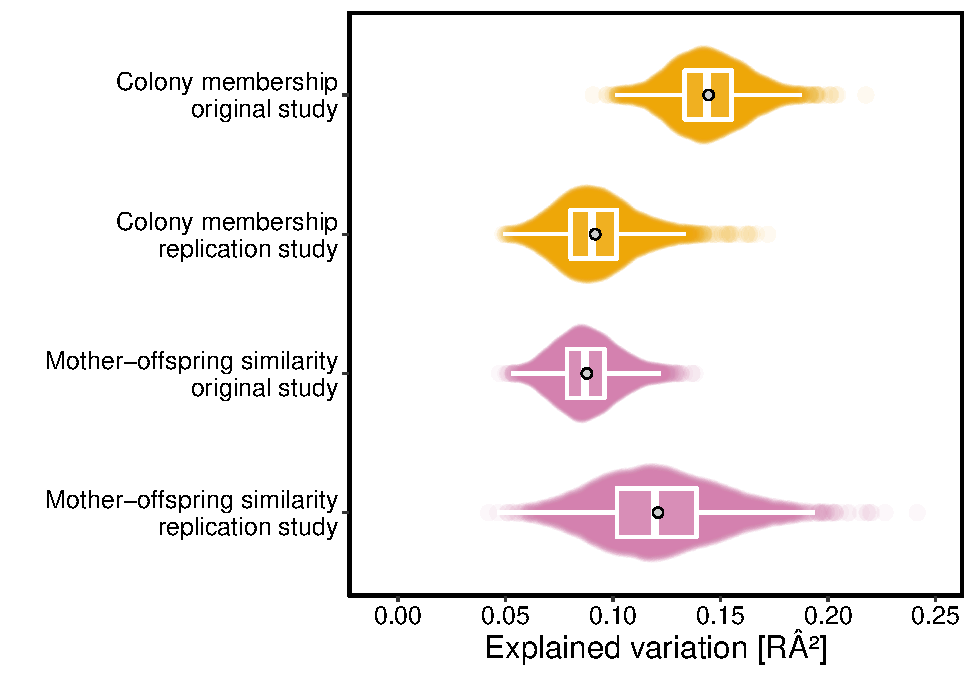
\includegraphics{SealScent_SI_Markdown_2020_1_files/figure-latex/Effect size estimate plot-1.pdf}

\subsection{R2 Bootstrap Code}\label{r2-bootstrap-code}

\begin{Shaded}
\begin{Highlighting}[]
\NormalTok{## creates function 'scent_btrap_r2_swarm_data' that performs bootstrap}

\CommentTok{# Bootstrap to track R2 values for randomized subsets. In addition,}
\CommentTok{# bootstrap cannot only be used to randomize the chemical data frame}
\CommentTok{# to evaluate R2 distribution as effect size estimates, }
\CommentTok{# but also to evaluate R2 change for different subsets based on different}
\CommentTok{# premises. 1) Frequent peaks 2) Strong concentrations 3) Peaks identified by SIMPER}

\KeywordTok{require}\NormalTok{(vegan)}

\CommentTok{# path: file path to scent_nmds-mompup2017_ssbfwb.RData", }
\CommentTok{#objects: scent_nmds, scent_nmds.obj, scent_factors, scent}
\CommentTok{# df.permutations: number of times the scent.df from loaded data will be permuted}
\CommentTok{# nmds.permutations: number of permutation in nMDS using Bray-Curtis}
\CommentTok{# btrap.iterations: number of procedure repeats}

\NormalTok{scent_btrap_r2_swarm_data <-}\StringTok{ }\ControlFlowTok{function}\NormalTok{(path, }\DataTypeTok{df.permutations =} \DecValTok{15}\NormalTok{, }
                                      \DataTypeTok{nmds.permutations =} \DecValTok{999}\NormalTok{, }
                                      \DataTypeTok{btrap.iterations =} \DecValTok{5000}\NormalTok{)\{}
  \CommentTok{# Create a data frame by permuting the data for scent}
  \CommentTok{# compounds data and also ensure that each population*age occur}
  \CommentTok{# same amounts of time in the permutation data frame. }
  \CommentTok{#---------------------------------------}
  
  \CommentTok{# load data frame with data of aligned fur seal chromatograms}
  \KeywordTok{load}\NormalTok{(path)}
\NormalTok{  scent_factors <-}\StringTok{ }\NormalTok{peak_factors}
  \CommentTok{# transfer BeachAge Column from scent_nmds to meta data.frame scent_factors}
\NormalTok{  scent_factors <-}\StringTok{ }\KeywordTok{cbind}\NormalTok{(scent_factors, }
                         \DataTypeTok{BeachAge =}\NormalTok{ scent_nmds}\OperatorTok{$}\NormalTok{BeachAge)}
  
  \CommentTok{# create index column for meta data frame}
\NormalTok{  scent_factors <-}\StringTok{ }\KeywordTok{cbind}\NormalTok{(scent_factors,}
                         \DataTypeTok{SampleIndex =} \DecValTok{1}\OperatorTok{:}\KeywordTok{length}\NormalTok{(}\KeywordTok{rownames}\NormalTok{(scent_factors)))}
  
  
  \CommentTok{# create data.frame to track PERMANOVA results over repeated tests}
\NormalTok{  nonsubset_results_paov <-}\StringTok{ }\KeywordTok{data.frame}\NormalTok{(}\DataTypeTok{R2_age =} \KeywordTok{double}\NormalTok{(), }\DataTypeTok{p_colfam =} \KeywordTok{double}\NormalTok{(),}
                                       \DataTypeTok{R2_residual =} \KeywordTok{double}\NormalTok{(), }
                                       \DataTypeTok{F_Het =} \KeywordTok{double}\NormalTok{(), }\DataTypeTok{p_Het =} \KeywordTok{double}\NormalTok{())}
\NormalTok{  promcomp_results_paov <-}\StringTok{ }\KeywordTok{data.frame}\NormalTok{(}\DataTypeTok{R2_age =} \KeywordTok{double}\NormalTok{(), }\DataTypeTok{p_colfam =} \KeywordTok{double}\NormalTok{(),}
                                      \DataTypeTok{R2_residual =} \KeywordTok{double}\NormalTok{(), }
                                      \DataTypeTok{F_Het =} \KeywordTok{double}\NormalTok{(), }\DataTypeTok{p_Het =} \KeywordTok{double}\NormalTok{())}
\NormalTok{  highcomp_results_paov <-}\StringTok{ }\KeywordTok{data.frame}\NormalTok{(}\DataTypeTok{R2_age =} \KeywordTok{double}\NormalTok{(), }\DataTypeTok{p_colfam =} \KeywordTok{double}\NormalTok{(),}
                                      \DataTypeTok{R2_residual =} \KeywordTok{double}\NormalTok{(), }
                                      \DataTypeTok{F_Het =} \KeywordTok{double}\NormalTok{(), }\DataTypeTok{p_Het =} \KeywordTok{double}\NormalTok{())}
\NormalTok{  simper_results_paov <-}\StringTok{ }\KeywordTok{data.frame}\NormalTok{(}\DataTypeTok{R2_age =} \KeywordTok{double}\NormalTok{(), }\DataTypeTok{p_colfam =} \KeywordTok{double}\NormalTok{(),}
                                    \DataTypeTok{R2_residual =} \KeywordTok{double}\NormalTok{(), }
                                    \DataTypeTok{F_Het =} \KeywordTok{double}\NormalTok{(), }\DataTypeTok{p_Het =} \KeywordTok{double}\NormalTok{())}
  
  \CommentTok{# create list to store created objects in an iteration}
\NormalTok{  iter_object_container <-}\StringTok{ }\KeywordTok{list}\NormalTok{()}
  
  \ControlFlowTok{for}\NormalTok{ (i }\ControlFlowTok{in} \DecValTok{1}\OperatorTok{:}\NormalTok{btrap.iterations) \{}
    
    
    \CommentTok{# create data.frame subsets (colony subset) by indexing the meta data.frame }
\NormalTok{    scent.f.ssb.m <-}\StringTok{ }\NormalTok{scent_factors[scent_factors}\OperatorTok{$}\NormalTok{BeachAge }\OperatorTok{==}\StringTok{ "SSB_1"}\NormalTok{,]}
\NormalTok{    scent.f.fwb.m <-}\StringTok{ }\NormalTok{scent_factors[scent_factors}\OperatorTok{$}\NormalTok{BeachAge }\OperatorTok{==}\StringTok{ "FWB_1"}\NormalTok{,]}
\NormalTok{    scent.f.ssb.p <-}\StringTok{ }\NormalTok{scent_factors[scent_factors}\OperatorTok{$}\NormalTok{BeachAge }\OperatorTok{==}\StringTok{ "SSB_2"}\NormalTok{,]}
\NormalTok{    scent.f.fwb.p <-}\StringTok{ }\NormalTok{scent_factors[scent_factors}\OperatorTok{$}\NormalTok{BeachAge }\OperatorTok{==}\StringTok{ "FWB_2"}\NormalTok{,]}
    
    \CommentTok{# int vector of row index number of permuted scent.ssb data.frame}
    \CommentTok{# row numbers will be used to create a permuted data.frame of }
    \CommentTok{# evenly distributed draws of individuals}
\NormalTok{    permute_rows_ssb_m <-}\StringTok{ }\KeywordTok{sample}\NormalTok{(scent.f.ssb.m}\OperatorTok{$}\NormalTok{SampleIndex, df.permutations, }\DataTypeTok{replace =}\NormalTok{ T)}
\NormalTok{    permute_rows_fwb_m <-}\StringTok{ }\KeywordTok{sample}\NormalTok{(scent.f.fwb.m}\OperatorTok{$}\NormalTok{SampleIndex, df.permutations, }\DataTypeTok{replace =}\NormalTok{ T)}
\NormalTok{    permute_rows_ssb_p <-}\StringTok{ }\KeywordTok{sample}\NormalTok{(scent.f.ssb.p}\OperatorTok{$}\NormalTok{SampleIndex, df.permutations, }\DataTypeTok{replace =}\NormalTok{ T)}
\NormalTok{    permute_rows_fwb_p <-}\StringTok{ }\KeywordTok{sample}\NormalTok{(scent.f.fwb.p}\OperatorTok{$}\NormalTok{SampleIndex, df.permutations, }\DataTypeTok{replace =}\NormalTok{ T)}
    
    \CommentTok{# create overall index number that can be used to }
    \CommentTok{#index data.frame(scent): index corresponds to correct individual }
\NormalTok{    perm_index_all <-}\StringTok{ }\KeywordTok{c}\NormalTok{(permute_rows_ssb_m, }
\NormalTok{                        permute_rows_fwb_m,}
\NormalTok{                        permute_rows_ssb_p,}
\NormalTok{                        permute_rows_fwb_p)}
    
    \CommentTok{# create new data.frame with indeces found in permutation }
    \CommentTok{# results vector perm_index_all}
\NormalTok{    scent.permute <-}\StringTok{ }\NormalTok{scent[perm_index_all,]}
\NormalTok{    scent_factors.permute <-}\StringTok{ }\NormalTok{scent_factors[perm_index_all,]}
    \CommentTok{# rownames(scent.permute) == rownames(scent_factors.permute) # TRUE}
    \CommentTok{#---------------------------------------}
    
    \CommentTok{# Perform analysis to find 3 subsets based on different premises }
    \CommentTok{# with the permuted data frame. }
    \CommentTok{# Track 15 best performing compounds of an analysis}
    \CommentTok{#---------------------------------------}
    
\NormalTok{    ## NDMS scale results}
\NormalTok{    ## count number of peaks that are not 0 per column}
\NormalTok{    peak_count <-}\StringTok{ }\KeywordTok{as.vector}\NormalTok{(}\KeywordTok{apply}\NormalTok{(scent.permute, }\DecValTok{2}\NormalTok{, }\ControlFlowTok{function}\NormalTok{(x) }\KeywordTok{length}\NormalTok{(x[x}\OperatorTok{>}\DecValTok{0}\NormalTok{]))) }
    
\NormalTok{    ## add peaks in a column that are not 0 to estimate highest }
    \CommentTok{# concentration peak sum}
\NormalTok{    peak_add <-}\StringTok{ }\KeywordTok{as.vector}\NormalTok{(}\KeywordTok{apply}\NormalTok{(scent.permute, }\DecValTok{2}\NormalTok{, }\ControlFlowTok{function}\NormalTok{(x) }\KeywordTok{sum}\NormalTok{(x))) }
    
\NormalTok{    ## create dataframe with same name properties as scent.RData}
\NormalTok{    compound_subset <-}\StringTok{ }\KeywordTok{data.frame}\NormalTok{(}\DataTypeTok{name =} \KeywordTok{colnames}\NormalTok{(scent.permute), }
\NormalTok{                                  peak_count, peak_add)}
    
\NormalTok{    ## sort data frame for most prominent compounds over all samples}
\NormalTok{    most_abundant <-}\StringTok{ }\NormalTok{compound_subset }\OperatorTok\StringTok{ }\KeywordTok{arrange}\NormalTok{(}\KeywordTok{desc}\NormalTok{(peak_count))}
    
\NormalTok{    ## shorten scent matrix to only the 15 most abundant compounds}
\NormalTok{    scent.promcomp <-}\StringTok{ }\NormalTok{scent.permute[}\KeywordTok{colnames}\NormalTok{(scent.permute) }\OperatorTok\StringTok{ }
\StringTok{                                      }\NormalTok{most_abundant}\OperatorTok{$}\NormalTok{name[}\DecValTok{1}\OperatorTok{:}\DecValTok{15}\NormalTok{]]}
    
\NormalTok{    ## sort data frame for most highly concentrated compounds over all samples}
\NormalTok{    most_concentration <-}\StringTok{ }\NormalTok{compound_subset }\OperatorTok\StringTok{ }\KeywordTok{arrange}\NormalTok{(}\KeywordTok{desc}\NormalTok{(peak_add))}
    
\NormalTok{    ## shorten scent matrix to only the 15 most abundant compounds}
\NormalTok{    scent.highcomp <-}\StringTok{ }\NormalTok{scent.permute[}\KeywordTok{colnames}\NormalTok{(scent.permute) }\OperatorTok\StringTok{ }
\StringTok{                                      }\NormalTok{most_concentration}\OperatorTok{$}\NormalTok{name[}\DecValTok{1}\OperatorTok{:}\DecValTok{15}\NormalTok{]]}
    
\NormalTok{    ## simper}
    \CommentTok{# simper analysis and results array}
\NormalTok{    sim <-}\StringTok{ }\KeywordTok{with}\NormalTok{(scent_factors.permute, }
                \KeywordTok{simper}\NormalTok{(scent.permute, colony))}
\NormalTok{    best.compounds.simper.btrap <-}\StringTok{ }\KeywordTok{summary}\NormalTok{(sim)[[}\DecValTok{1}\NormalTok{]]}
    \CommentTok{#filter 15 compounds that contribute most towards dissimilarity of individuals}
\NormalTok{    simper_comps <-}\StringTok{ }\KeywordTok{as.numeric}\NormalTok{(}\KeywordTok{rownames}\NormalTok{(best.compounds.simper.btrap))}
\NormalTok{    best_comps <-}\StringTok{ }\NormalTok{simper_comps[}\DecValTok{1}\OperatorTok{:}\DecValTok{15}\NormalTok{] }
    \CommentTok{# subset peak data matrix \{scent\}}
\NormalTok{    scent.simper.btrap <-}\StringTok{ }\NormalTok{scent.permute[,}\KeywordTok{which}\NormalTok{(}\KeywordTok{colnames}\NormalTok{(scent.permute) }\OperatorTok\StringTok{ }
\StringTok{                                                 }\KeywordTok{as.character}\NormalTok{(best_comps))]}
    \CommentTok{#---------------------------------------}
    
    \CommentTok{# Take 15 identified compounds and limit nMDS of the permuted }
    \CommentTok{# data frame (scent.permute) to only those compounds}
    
    \CommentTok{#---------------------------------------}
    
    \CommentTok{# bray-curtis similarity}
\NormalTok{    scent_nmds_regular.obj <-}\StringTok{ }\NormalTok{vegan}\OperatorTok{::}\KeywordTok{metaMDS}\NormalTok{(}\DataTypeTok{comm =}\NormalTok{ scent.permute, }\DataTypeTok{k =} \DecValTok{2}\NormalTok{, }
                                             \DataTypeTok{try =}\NormalTok{ df.permutations, }\DataTypeTok{distance =} \StringTok{"bray"}\NormalTok{)}
\NormalTok{    scent_nmds_count.obj <-}\StringTok{ }\NormalTok{vegan}\OperatorTok{::}\KeywordTok{metaMDS}\NormalTok{(}\DataTypeTok{comm =}\NormalTok{ scent.promcomp, }\DataTypeTok{k =} \DecValTok{2}\NormalTok{, }
                                           \DataTypeTok{try =}\NormalTok{ df.permutations, }\DataTypeTok{distance =} \StringTok{"bray"}\NormalTok{) }
\NormalTok{    scent_nmds_add.obj <-}\StringTok{ }\NormalTok{vegan}\OperatorTok{::}\KeywordTok{metaMDS}\NormalTok{(}\DataTypeTok{comm =}\NormalTok{ scent.highcomp, }\DataTypeTok{k =} \DecValTok{2}\NormalTok{, }
                                         \DataTypeTok{try =}\NormalTok{ df.permutations, }\DataTypeTok{distance =} \StringTok{"bray"}\NormalTok{) }
\NormalTok{    scent_nmds_simper.obj <-}\StringTok{ }\NormalTok{vegan}\OperatorTok{::}\KeywordTok{metaMDS}\NormalTok{(}\DataTypeTok{comm =}\NormalTok{ scent.simper.btrap, }\DataTypeTok{k =} \DecValTok{2}\NormalTok{, }
                                            \DataTypeTok{try =}\NormalTok{ df.permutations, }\DataTypeTok{distance =} \StringTok{"bray"}\NormalTok{)}
    
\NormalTok{    ## get x and y coordinates}
\NormalTok{    scent_nmds_regular <-}\StringTok{ }\KeywordTok{as.data.frame}\NormalTok{(scent_nmds_regular.obj[[}\StringTok{"points"}\NormalTok{]])}
\NormalTok{    scent_nmds_count <-}\StringTok{ }\KeywordTok{as.data.frame}\NormalTok{(scent_nmds_count.obj[[}\StringTok{"points"}\NormalTok{]]) }
\NormalTok{    scent_nmds_add <-}\StringTok{ }\KeywordTok{as.data.frame}\NormalTok{(scent_nmds_add.obj[[}\StringTok{"points"}\NormalTok{]])}
\NormalTok{    scent_nmds_simper <-}\StringTok{ }\KeywordTok{as.data.frame}\NormalTok{(scent_nmds_simper.obj[[}\StringTok{"points"}\NormalTok{]])}
    
\NormalTok{    ## add the colony as a factor to each sample}
\NormalTok{    scent_nmds <-}\StringTok{ }\KeywordTok{data.frame}\NormalTok{(}\DataTypeTok{MDS1r =}\NormalTok{ scent_nmds_regular[[}\StringTok{"MDS1"}\NormalTok{]],}
                             \DataTypeTok{MDS2r =}\NormalTok{ scent_nmds_regular[[}\StringTok{"MDS2"}\NormalTok{]],}
                             \DataTypeTok{MDS1c =}\NormalTok{ scent_nmds_count[[}\StringTok{"MDS1"}\NormalTok{]],}
                             \DataTypeTok{MDS2c =}\NormalTok{ scent_nmds_count[[}\StringTok{"MDS2"}\NormalTok{]],}
                             \DataTypeTok{MDS1a =}\NormalTok{ scent_nmds_add[[}\StringTok{"MDS1"}\NormalTok{]],}
                             \DataTypeTok{MDS2a =}\NormalTok{ scent_nmds_add[[}\StringTok{"MDS2"}\NormalTok{]],}
                             \DataTypeTok{MDS1s =}\NormalTok{ scent_nmds_simper[[}\StringTok{"MDS1"}\NormalTok{]],}
                             \DataTypeTok{MDS2s =}\NormalTok{ scent_nmds_simper[[}\StringTok{"MDS2"}\NormalTok{]], }
                             \DataTypeTok{age =}\NormalTok{ scent_factors.permute[[}\StringTok{"age"}\NormalTok{]],}
                             \DataTypeTok{colony =}\NormalTok{ scent_factors.permute[[}\StringTok{"colony"}\NormalTok{]],}
                             \DataTypeTok{family =}\NormalTok{ scent_factors.permute[[}\StringTok{"family"}\NormalTok{]],}
                             \DataTypeTok{BeachAge =}\NormalTok{ scent_factors.permute[[}\StringTok{"BeachAge"}\NormalTok{]]}
\NormalTok{    )}
    \CommentTok{#---------------------------------------}
    
    \CommentTok{# Perform PERMANOVA on distance matrix based limited scent compounds data}
    \CommentTok{#---------------------------------------}
    
    \CommentTok{# not subsetted}
\NormalTok{    nonsubset.df_permanova <-}\StringTok{ }\KeywordTok{adonis}\NormalTok{(scent.permute }\OperatorTok{~}\StringTok{ }\NormalTok{age }\OperatorTok{+}\StringTok{ }\NormalTok{colony }\OperatorTok{+}\StringTok{ }\NormalTok{colony}\OperatorTok{:}\NormalTok{family,}
                                     \DataTypeTok{data =}\NormalTok{ scent_factors.permute,}
                                     \DataTypeTok{permutations =} \DecValTok{9999}\NormalTok{)}
\NormalTok{    nonsubset.df_hetgeneity <-}\StringTok{ }\KeywordTok{anova}\NormalTok{(}\KeywordTok{betadisper}\NormalTok{(}\KeywordTok{vegdist}\NormalTok{(scent.permute), }
\NormalTok{                                                scent_factors.permute}\OperatorTok{$}\NormalTok{colony))}
    
    \CommentTok{# track important values of statistical analysis in this run}
\NormalTok{    nonsubset_iter_res_paov <-}\StringTok{ }\KeywordTok{cbind}\NormalTok{(}\DataTypeTok{R2_age =}\NormalTok{ nonsubset.df_permanova}\OperatorTok{$}\NormalTok{aov.tab}\OperatorTok{$}\NormalTok{R2[}\DecValTok{1}\NormalTok{],}
                                     \DataTypeTok{R2_colony =}\NormalTok{ nonsubset.df_permanova}\OperatorTok{$}\NormalTok{aov.tab}\OperatorTok{$}\NormalTok{R2[}\DecValTok{2}\NormalTok{],}
                                     \DataTypeTok{R2_famcol =}\NormalTok{ nonsubset.df_permanova}\OperatorTok{$}\NormalTok{aov.tab}\OperatorTok{$}\NormalTok{R2[}\DecValTok{3}\NormalTok{],}
                                     \DataTypeTok{R2_residual =}\NormalTok{ nonsubset.df_permanova}\OperatorTok{$}\NormalTok{aov.tab}\OperatorTok{$}\NormalTok{R2[}\DecValTok{4}\NormalTok{],}
                                     \DataTypeTok{F_Het =}\NormalTok{ nonsubset.df_hetgeneity}\OperatorTok{$}\StringTok{`}\DataTypeTok{F value}\StringTok{`}\NormalTok{[}\DecValTok{1}\NormalTok{],}
                                     \DataTypeTok{p_Het =}\NormalTok{ nonsubset.df_hetgeneity}\OperatorTok{$}\StringTok{`}\DataTypeTok{Pr(>F)}\StringTok{`}\NormalTok{[}\DecValTok{1}\NormalTok{])}
    
    \CommentTok{# bind run values to track changes over iterations in the for-loop}
\NormalTok{    nonsubset_results_paov <-}\StringTok{ }\KeywordTok{rbind}\NormalTok{(nonsubset_results_paov,}
\NormalTok{                                    nonsubset_iter_res_paov)}
  
    \CommentTok{#prom comps}
\NormalTok{    promcomp.df_permanova <-}\StringTok{ }\KeywordTok{adonis}\NormalTok{(scent.promcomp }\OperatorTok{~}\StringTok{ }\NormalTok{age }\OperatorTok{+}\StringTok{ }\NormalTok{colony }\OperatorTok{+}\StringTok{ }\NormalTok{colony}\OperatorTok{:}\NormalTok{family, }
                                    \DataTypeTok{data =}\NormalTok{ scent_factors.permute, }
                                    \DataTypeTok{permutations =} \DecValTok{9999}\NormalTok{) }
\NormalTok{    promcomp.df_hetgeneity <-}\StringTok{ }\KeywordTok{anova}\NormalTok{(}\KeywordTok{betadisper}\NormalTok{(}\KeywordTok{vegdist}\NormalTok{(scent.promcomp), }
\NormalTok{                                               scent_factors.permute}\OperatorTok{$}\NormalTok{colony)) }
    
\NormalTok{    promcomp_iter_res_paov <-}\StringTok{ }\KeywordTok{cbind}\NormalTok{(}\DataTypeTok{R2_age =}\NormalTok{ promcomp.df_permanova}\OperatorTok{$}\NormalTok{aov.tab}\OperatorTok{$}\NormalTok{R2[}\DecValTok{1}\NormalTok{],}
                                    \DataTypeTok{R2_colony =}\NormalTok{ promcomp.df_permanova}\OperatorTok{$}\NormalTok{aov.tab}\OperatorTok{$}\NormalTok{R2[}\DecValTok{2}\NormalTok{],}
                                    \DataTypeTok{R2_famcol =}\NormalTok{ promcomp.df_permanova}\OperatorTok{$}\NormalTok{aov.tab}\OperatorTok{$}\NormalTok{R2[}\DecValTok{3}\NormalTok{],}
                                    \DataTypeTok{R2_residual =}\NormalTok{ promcomp.df_permanova}\OperatorTok{$}\NormalTok{aov.tab}\OperatorTok{$}\NormalTok{R2[}\DecValTok{4}\NormalTok{],}
                                    \DataTypeTok{F_Het =}\NormalTok{ promcomp.df_hetgeneity}\OperatorTok{$}\StringTok{`}\DataTypeTok{F value}\StringTok{`}\NormalTok{[}\DecValTok{1}\NormalTok{],}
                                    \DataTypeTok{p_Het =}\NormalTok{ promcomp.df_hetgeneity}\OperatorTok{$}\StringTok{`}\DataTypeTok{Pr(>F)}\StringTok{`}\NormalTok{[}\DecValTok{1}\NormalTok{])}
    
\NormalTok{    promcomp_results_paov <-}\StringTok{ }\KeywordTok{rbind}\NormalTok{(promcomp_results_paov,}
\NormalTok{                                   promcomp_iter_res_paov)}
    
    \CommentTok{# high comps}
\NormalTok{    highcomp.df_permanova <-}\StringTok{ }\KeywordTok{adonis}\NormalTok{(scent.highcomp }\OperatorTok{~}\StringTok{ }\NormalTok{age }\OperatorTok{+}\StringTok{ }\NormalTok{colony }\OperatorTok{+}\StringTok{ }\NormalTok{colony}\OperatorTok{:}\NormalTok{family, }
                                    \DataTypeTok{data =}\NormalTok{ scent_factors.permute, }
                                    \DataTypeTok{permutations =} \DecValTok{9999}\NormalTok{) }
\NormalTok{    highcomp.df_hetgeneity <-}\StringTok{ }\KeywordTok{anova}\NormalTok{(}\KeywordTok{betadisper}\NormalTok{(}\KeywordTok{vegdist}\NormalTok{(scent.highcomp), scent_factors.permute}\OperatorTok{$}\NormalTok{colony)) }
    
\NormalTok{    highcomp_iter_res_paov <-}\StringTok{ }\KeywordTok{cbind}\NormalTok{(}\DataTypeTok{R2_age =}\NormalTok{ highcomp.df_permanova}\OperatorTok{$}\NormalTok{aov.tab}\OperatorTok{$}\NormalTok{R2[}\DecValTok{1}\NormalTok{],}
                                    \DataTypeTok{R2_colony =}\NormalTok{ highcomp.df_permanova}\OperatorTok{$}\NormalTok{aov.tab}\OperatorTok{$}\NormalTok{R2[}\DecValTok{2}\NormalTok{],}
                                    \DataTypeTok{R2_famcol =}\NormalTok{ highcomp.df_permanova}\OperatorTok{$}\NormalTok{aov.tab}\OperatorTok{$}\NormalTok{R2[}\DecValTok{3}\NormalTok{],}
                                    \DataTypeTok{R2_residual =}\NormalTok{ highcomp.df_permanova}\OperatorTok{$}\NormalTok{aov.tab}\OperatorTok{$}\NormalTok{R2[}\DecValTok{4}\NormalTok{],}
                                    \DataTypeTok{F_Het =}\NormalTok{ highcomp.df_hetgeneity}\OperatorTok{$}\StringTok{`}\DataTypeTok{F value}\StringTok{`}\NormalTok{[}\DecValTok{1}\NormalTok{],}
                                    \DataTypeTok{p_Het =}\NormalTok{ highcomp.df_hetgeneity}\OperatorTok{$}\StringTok{`}\DataTypeTok{Pr(>F)}\StringTok{`}\NormalTok{[}\DecValTok{1}\NormalTok{])}
    
\NormalTok{    highcomp_results_paov <-}\StringTok{ }\KeywordTok{rbind}\NormalTok{(highcomp_results_paov,}
\NormalTok{                                   highcomp_iter_res_paov)}
    \CommentTok{# SIMPER}
\NormalTok{    simper.df_permanova <-}\StringTok{ }\KeywordTok{adonis}\NormalTok{(scent.simper.btrap }\OperatorTok{~}\StringTok{ }\NormalTok{age }\OperatorTok{+}\StringTok{ }\NormalTok{colony }\OperatorTok{+}\StringTok{ }\NormalTok{colony}\OperatorTok{:}\NormalTok{family, }
                                  \DataTypeTok{data =}\NormalTok{ scent_factors.permute, }
                                  \DataTypeTok{permutations =} \DecValTok{9999}\NormalTok{) }
\NormalTok{    simper.df_hetgeneity <-}\StringTok{ }\KeywordTok{anova}\NormalTok{(}\KeywordTok{betadisper}\NormalTok{(}\KeywordTok{vegdist}\NormalTok{(scent.simper.btrap), scent_factors.permute}\OperatorTok{$}\NormalTok{colony)) }
    
\NormalTok{    simper_iter_res_paov <-}\StringTok{ }\KeywordTok{cbind}\NormalTok{(}\DataTypeTok{R2_age =}\NormalTok{ simper.df_permanova}\OperatorTok{$}\NormalTok{aov.tab}\OperatorTok{$}\NormalTok{R2[}\DecValTok{1}\NormalTok{],}
                                  \DataTypeTok{R2_colony =}\NormalTok{ simper.df_permanova}\OperatorTok{$}\NormalTok{aov.tab}\OperatorTok{$}\NormalTok{R2[}\DecValTok{2}\NormalTok{],}
                                  \DataTypeTok{R2_famcol =}\NormalTok{ simper.df_permanova}\OperatorTok{$}\NormalTok{aov.tab}\OperatorTok{$}\NormalTok{R2[}\DecValTok{3}\NormalTok{],}
                                  \DataTypeTok{R2_residual =}\NormalTok{ simper.df_permanova}\OperatorTok{$}\NormalTok{aov.tab}\OperatorTok{$}\NormalTok{R2[}\DecValTok{4}\NormalTok{],}
                                  \DataTypeTok{F_Het =}\NormalTok{ simper.df_hetgeneity}\OperatorTok{$}\StringTok{`}\DataTypeTok{F value}\StringTok{`}\NormalTok{[}\DecValTok{1}\NormalTok{],}
                                  \DataTypeTok{p_Het =}\NormalTok{ simper.df_hetgeneity}\OperatorTok{$}\StringTok{`}\DataTypeTok{Pr(>F)}\StringTok{`}\NormalTok{[}\DecValTok{1}\NormalTok{])}
    
\NormalTok{    simper_results_paov <-}\StringTok{ }\KeywordTok{rbind}\NormalTok{(simper_results_paov,}
\NormalTok{                                 simper_iter_res_paov)}
    \CommentTok{#---------------------------------------}
    
    
    \CommentTok{# # pack all this in a list to be later on stored in a list that can be saved again}
    \CommentTok{# create name giving the iteration step}
\NormalTok{    iteration_count <-}\StringTok{ }\KeywordTok{paste0}\NormalTok{(}\StringTok{"iter_"}\NormalTok{, i)}
    
    \CommentTok{# create list that stores relevant workspace elements for an iteration step}
\NormalTok{    iter_objects <-}\StringTok{ }\KeywordTok{list}\NormalTok{(}\DataTypeTok{scent.permute =}\NormalTok{ scent.permute,}
                         \DataTypeTok{scent_factors.permute =}\NormalTok{ scent_factors.permute,}
                         \DataTypeTok{scent.promcomp =}\NormalTok{ scent.promcomp,}
                         \DataTypeTok{scent.highcomp =}\NormalTok{ scent.highcomp,}
                         \DataTypeTok{sim =}\NormalTok{ sim,}
                         \DataTypeTok{scent.simper.btrap =}\NormalTok{ scent.simper.btrap,}
                         \DataTypeTok{scent_nmds_regular.obj =}\NormalTok{ scent_nmds_regular.obj,}
                         \DataTypeTok{scent_nmds_count.obj =}\NormalTok{ scent_nmds_count.obj,}
                         \DataTypeTok{scent_nmds_add.obj =}\NormalTok{ scent_nmds_add.obj,}
                         \DataTypeTok{scent_nmds_simper.obj =}\NormalTok{ scent_nmds_simper.obj,}
                         \DataTypeTok{scent_nmds_regular =}\NormalTok{ scent_nmds_regular,}
                         \DataTypeTok{scent_nmds_count =}\NormalTok{ scent_nmds_count,}
                         \DataTypeTok{scent_nmds_add =}\NormalTok{ scent_nmds_add,}
                         \DataTypeTok{scent_nmds_simper =}\NormalTok{ scent_nmds_simper,}
                         \DataTypeTok{promcomp.df_permanova =}\NormalTok{ promcomp.df_permanova,}
                         \DataTypeTok{promcomp.df_hetgeneity =}\NormalTok{ promcomp.df_hetgeneity,}
                         \DataTypeTok{highcomp.df_permanova =}\NormalTok{ highcomp.df_permanova,}
                         \DataTypeTok{highcomp.df_hetgeneity =}\NormalTok{ highcomp.df_permanova,}
                         \DataTypeTok{simper.df_permanova =}\NormalTok{ simper.df_permanova,}
                         \DataTypeTok{simper.df_hetgeneity =}\NormalTok{ simper.df_hetgeneity)}
    
    \CommentTok{# save everything as a list in a container list, that stores }
    \CommentTok{# information/elements of all iteration steps}
\NormalTok{    iter_object_container[[i]] <-}\StringTok{ }\NormalTok{iter_objects}
    \KeywordTok{names}\NormalTok{(iter_object_container)[i] <-}\StringTok{ }\NormalTok{iteration_count}
    
\NormalTok{  \} }\CommentTok{# end i}
  
\NormalTok{  paov_r2_results <-}\StringTok{ }\KeywordTok{list}\NormalTok{(}\DataTypeTok{regular =}\NormalTok{ nonsubset_results_paov,}
                          \DataTypeTok{promcomp =}\NormalTok{ promcomp_results_paov,}
                          \DataTypeTok{highcomp =}\NormalTok{ highcomp_results_paov,}
                          \DataTypeTok{simper_res =}\NormalTok{ simper_results_paov)}
  \KeywordTok{return}\NormalTok{(}\KeywordTok{list}\NormalTok{(}\DataTypeTok{paov_r2_results =}\NormalTok{ paov_r2_results, }
              \DataTypeTok{iter_object_container =}\NormalTok{ iter_object_container))}
\NormalTok{\} }\CommentTok{# end function}
\end{Highlighting}
\end{Shaded}

\subsection{Session information}\label{session-information}

\begin{verbatim}
## R version 3.5.3 (2019-03-11)
## Platform: x86_64-w64-mingw32/x64 (64-bit)
## Running under: Windows 10 x64 (build 18363)
## 
## Matrix products: default
## 
## locale:
## [1] LC_COLLATE=English_Germany.1252  LC_CTYPE=English_Germany.1252   
## [3] LC_MONETARY=English_Germany.1252 LC_NUMERIC=C                    
## [5] LC_TIME=English_Germany.1252    
## 
## attached base packages:
## [1] stats     graphics  grDevices utils     datasets  methods   base     
## 
## other attached packages:
##  [1] pairwiseAdonis_0.0.1 cluster_2.0.7-1      forcats_0.4.0       
##  [4] stringr_1.4.0        dplyr_0.8.0.1        purrr_0.3.1         
##  [7] tidyr_0.8.3          tibble_2.0.1         tidyverse_1.2.1     
## [10] ggbeeswarm_0.6.0     ggplot2_3.1.1        readr_1.3.1         
## [13] vegan_2.5-4          lattice_0.20-38      permute_0.9-5       
## [16] GCalignR_1.0.2      
## 
## loaded via a namespace (and not attached):
##  [1] Rcpp_1.0.0       lubridate_1.7.4  assertthat_0.2.0 digest_0.6.18   
##  [5] R6_2.4.0         cellranger_1.1.0 plyr_1.8.4       backports_1.1.3 
##  [9] evaluate_0.13    httr_1.4.0       pillar_1.3.1     rlang_0.3.1     
## [13] lazyeval_0.2.1   readxl_1.3.0     rstudioapi_0.9.0 Matrix_1.2-15   
## [17] rmarkdown_2.1    labeling_0.3     splines_3.5.3    munsell_0.5.0   
## [21] broom_0.5.1      compiler_3.5.3   vipor_0.4.5      modelr_0.1.4    
## [25] xfun_0.5         pkgconfig_2.0.2  mgcv_1.8-27      htmltools_0.3.6 
## [29] tidyselect_0.2.5 crayon_1.3.4     withr_2.1.2      MASS_7.3-51.1   
## [33] grid_3.5.3       nlme_3.1-137     jsonlite_1.6     gtable_0.2.0    
## [37] magrittr_1.5     scales_1.0.0     cli_1.0.1        stringi_1.3.1   
## [41] xml2_1.2.0       generics_0.0.2   tools_3.5.3      glue_1.3.0      
## [45] beeswarm_0.2.3   hms_0.4.2        parallel_3.5.3   yaml_2.2.0      
## [49] colorspace_1.4-0 rvest_0.3.2      knitr_1.22       haven_2.1.0
\end{verbatim}

\end{document}
